\section{Inter-domain Routing Protocol: BGP}
\label{sec:bgp}

\subsection{Design}
For inter-domain routing, Border Gateway Protocol (BGP)\citep{rfc4271} is applied in BT Network since it's the one and only External Gateway Protocol (EGP) in today's global Internet. BGP provides scaliability to large networks, clear definations of administrative boudnary as well as flexiable policy control, which allow business relaitonships with neighbouring ISPs to be expressed in terms of routing policies.

Figure \ref{fig:bgp} shows the design of BGP protocol in our network. The AS Number (ASN) of BT Network is 2030 while ASN of Central, Virgin, DT are 42, 5060, 3040 respectively. 

\begin{figure}[ht!]
    \centering
    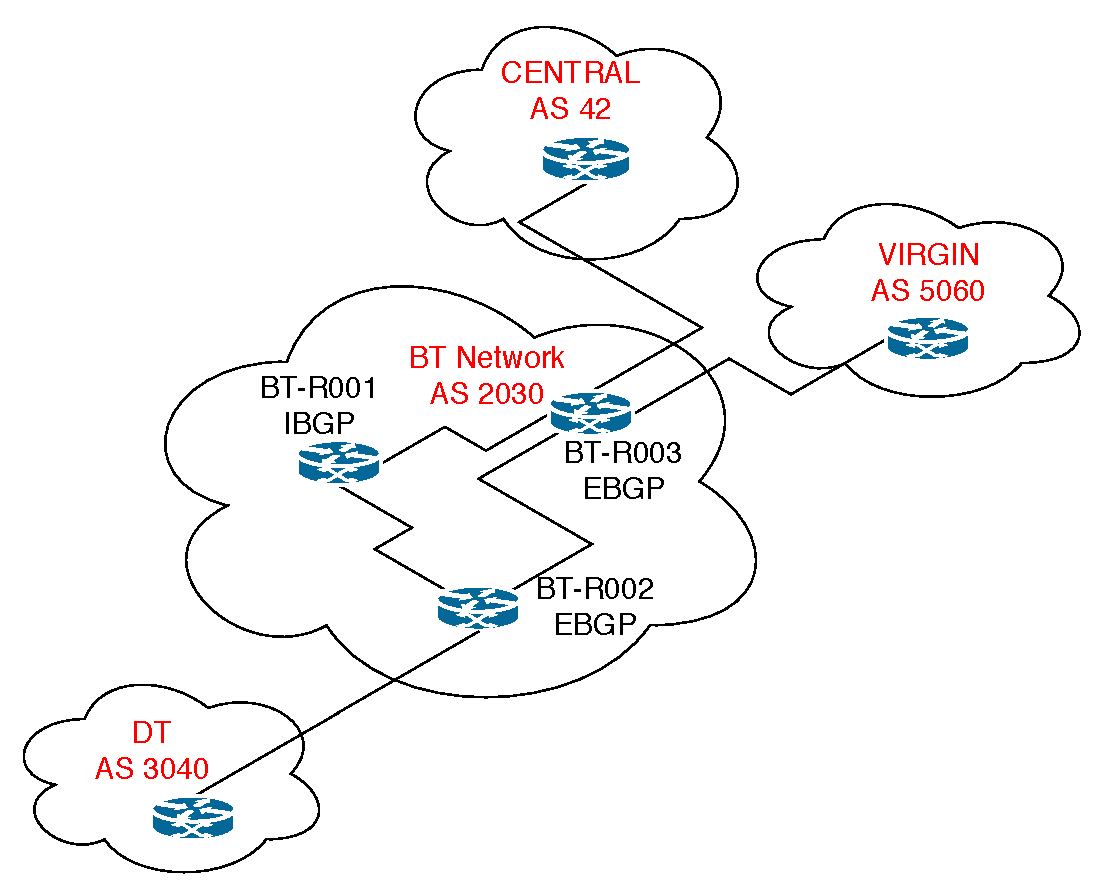
\includegraphics[width=\linewidth]{bgp}
    \caption{Design of BGP Protocol in BT Network.}
    \label{fig:bgp}
\end{figure}

Router 2 (BT-R002) and Router 3 (BT-R003) act as External BGP routers since they are directly connected to neighbouring ISPs. They receive routes announced by neighbouring ISPs' routers and announce routes originated from BT Network.
Router 1 (BT-R001) acts as an Internal BGP (IBGP) router only since it is not directly connected to any neighbouring ISP and only forwards and receives routes announced by EGBP routers.




\subsection{Routing Policies}

To enact business relationships with neighbouring ISPs, proper routing polices should be implemented for each different relationship in BGP protocol. 
Specifically, for customer ISPs, all routes announced by such ISP should be accepted and all routes received should be annouced to it as well. This allows customers to connect to BT Network as well as connect to other networks through BT Network.

For non-customer neighbouring ISPs (peers and providers), all routes announced by such ISP should be accepted in order for BT Network to connect to it. Meanwhile, only routes originated from either BT Network or BT's customers are announced to such ISP.

\subsection{Implementation}

On Router 1 (BT-R001, IPv4 Loopback Address: \texttt{23.0.255.1}, IPv6 Loopback Address: \texttt{2001:2300:FFFF:1::}), both Router 2 (BT-R002, IPv4 Loopback Address: \texttt{23.0.255.2}, IPv6 Loopback Address: \texttt{2001:2300:FFFF:2::}) and Router 3 (BT-R003, IPv4 Loopback Address: \texttt{23.0.255.3}, IPv6 Loopback Address: \texttt{2001:2300:FFFF:3::}) are taken as neighbouring routers in the same AS.
In addition, the source of BGP messages are set to be the loopback address of Router 1 to prevent physical disconnection to the $2$ routers.
Router 1 announces the subnet \texttt{BT-R001 - BT001} (IPv4: \texttt{23.0.0.0/28}, IPv6: \texttt{2001:2300:0:0::/64}) to other routers.

\begin{lstlisting}
router bgp 2030
network 23.0.0.0 mask 255.255.255.240
neighbor 23.0.255.2 remote-as 2030
neighbor 23.0.255.2 update-source Loopback0
neighbor 23.0.255.3 remote-as 2030
neighbor 23.0.255.3 update-source Loopback0
neighbor 2001:2300:FFFF:2:: remote-as 2030
neighbor 2001:2300:FFFF:2:: update-source Loopback0
neighbor 2001:2300:FFFF:3:: remote-as 2030
neighbor 2001:2300:FFFF:3:: update-source Loopback0

address-family ipv6
network 2001:2300::/64
neighbor 2001:2300:FFFF:2:: activate
neighbor 2001:2300:FFFF:3:: activate
\end{lstlisting}

On Router 2 (BT-R002), both Router 1 and Router 3 are taken as neighbouring routers in the same AS while the router from DT is taken as router from AS 3040.
Router 2 announces the subnet \texttt{BT-R002 - BT002} (IPv4: \texttt{23.0.0.16/28}, IPv6: \texttt{2001:2300:0:1::/64}) to other routers.
Since Router 2 is direclty connected to customer DT Network, it applies no filter on inbound and outbound routes.

\begin{lstlisting}
router bgp 2030
network 23.0.0.16 mask 255.255.255.240
neighbor 23.0.0.62 remote-as 3040
neighbor 23.0.255.1 remote-as 2030
neighbor 23.0.255.1 update-source Loopback0
neighbor 23.0.255.3 remote-as 2030
neighbor 23.0.255.3 update-source Loopback0
neighbor 2001:2300:0:6::2 remote-as 3040
neighbor 2001:2300:FFFF:1:: remote-as 2030
neighbor 2001:2300:FFFF:1:: update-source Loopback0
neighbor 2001:2300:FFFF:3:: remote-as 2030
neighbor 2001:2300:FFFF:3:: update-source Loopback0

address-family ipv6
network 2001:2300:0:1::/64
neighbor 2001:2300:0:6::2 activate
neighbor 2001:2300:FFFF:1:: activate
neighbor 2001:2300:FFFF:3:: activate
\end{lstlisting}

On Router 3 (BT-R003), both Router 1 and Router 2 are taken as neighbouring routers in the same AS while the routers from Central and Virgin are taken as router from AS 42 and AS 5060 respectively.
Router 3 announces the subnet \texttt{BT-R003 - BT003} (IPv4: \texttt{23.0.0.32/28}, IPv6: \texttt{2001:2300:0:2::/64}) to other routers.

\begin{lstlisting}
router bgp 2030
network 23.0.0.32 mask 255.255.255.240
neighbor 23.0.255.1 remote-as 2030
neighbor 23.0.255.1 update-source Loopback0
neighbor 23.0.255.2 remote-as 2030
neighbor 23.0.255.2 update-source Loopback0
neighbor 2001:2300:FFFF:1:: remote-as 2030
neighbor 2001:2300:FFFF:1:: update-source Loopback0
neighbor 2001:2300:FFFF:2:: remote-as 2030
neighbor 2001:2300:FFFF:2:: update-source Loopback0
neighbor 2001:5600:0:6::1 remote-as 5060
neighbor 56.0.0.61 remote-as 5060
neighbor 100.100.2.1 remote-as 42

address-family ipv6
network 2001:2300:0:2::/64
aggregate-address 2001:2300::/32 summary-only
neighbor 2001:2300:FFFF:1:: activate
neighbor 2001:2300:FFFF:2:: activate
\end{lstlisting}


Since Router 3 is direclty connected to non-customer ISPs, it applies a filter on outbound routes, which denies all routes that pass through either Central Network (ASN: $42$) or Virgin Network (ASN: $5060$).

\begin{lstlisting}
ip as-path access-list 1 deny _42_
ip as-path access-list 1 deny _5060_
ip as-path access-list 1 permit .*
router bgp 2030
neighbor 56.0.0.61 filter-list 1 out
neighbor 100.100.2.1 filter-list 1 out
\end{lstlisting}

Address aggregation for \texttt{23.0.0.0/8} and \texttt{2001:2300::/32} is set up on all 3 routers, which aggregates routes destined for all addresses inside BT Network range into a single route.

\begin{lstlisting}
aggregate-address 23.0.0.0 255.0.0.0 summary-only
address-family ipv6
aggregate-address 2001:2300::/32 summary-only
\end{lstlisting}


\subsection{Evaluation}

\subsubsection{BGP Routes}

Routes collected through BGP protocol on all $3$ routers are shown in Figure \ref{fig:bgp-route} and \ref{fig:bgp-route-ipv6} using commands \texttt{show bgp} and \texttt{show bgp ipv6}. 
Routes to DT Network (IPv4: \texttt{34.0.0.0/8}, IPv6: \texttt{2001:3400::/32}), Virgin Network (IPv4: \texttt{56.0.0.0/8}, IPv6: \texttt{2001:5600::/32}), Central Network (IPv4: \texttt{10.2.2.0/24}) and other networks can be observed in the figure.

\begin{figure*}[ht!]
    \centering
    \begin{subfigure}[b]{0.67\textwidth}
        \centering
        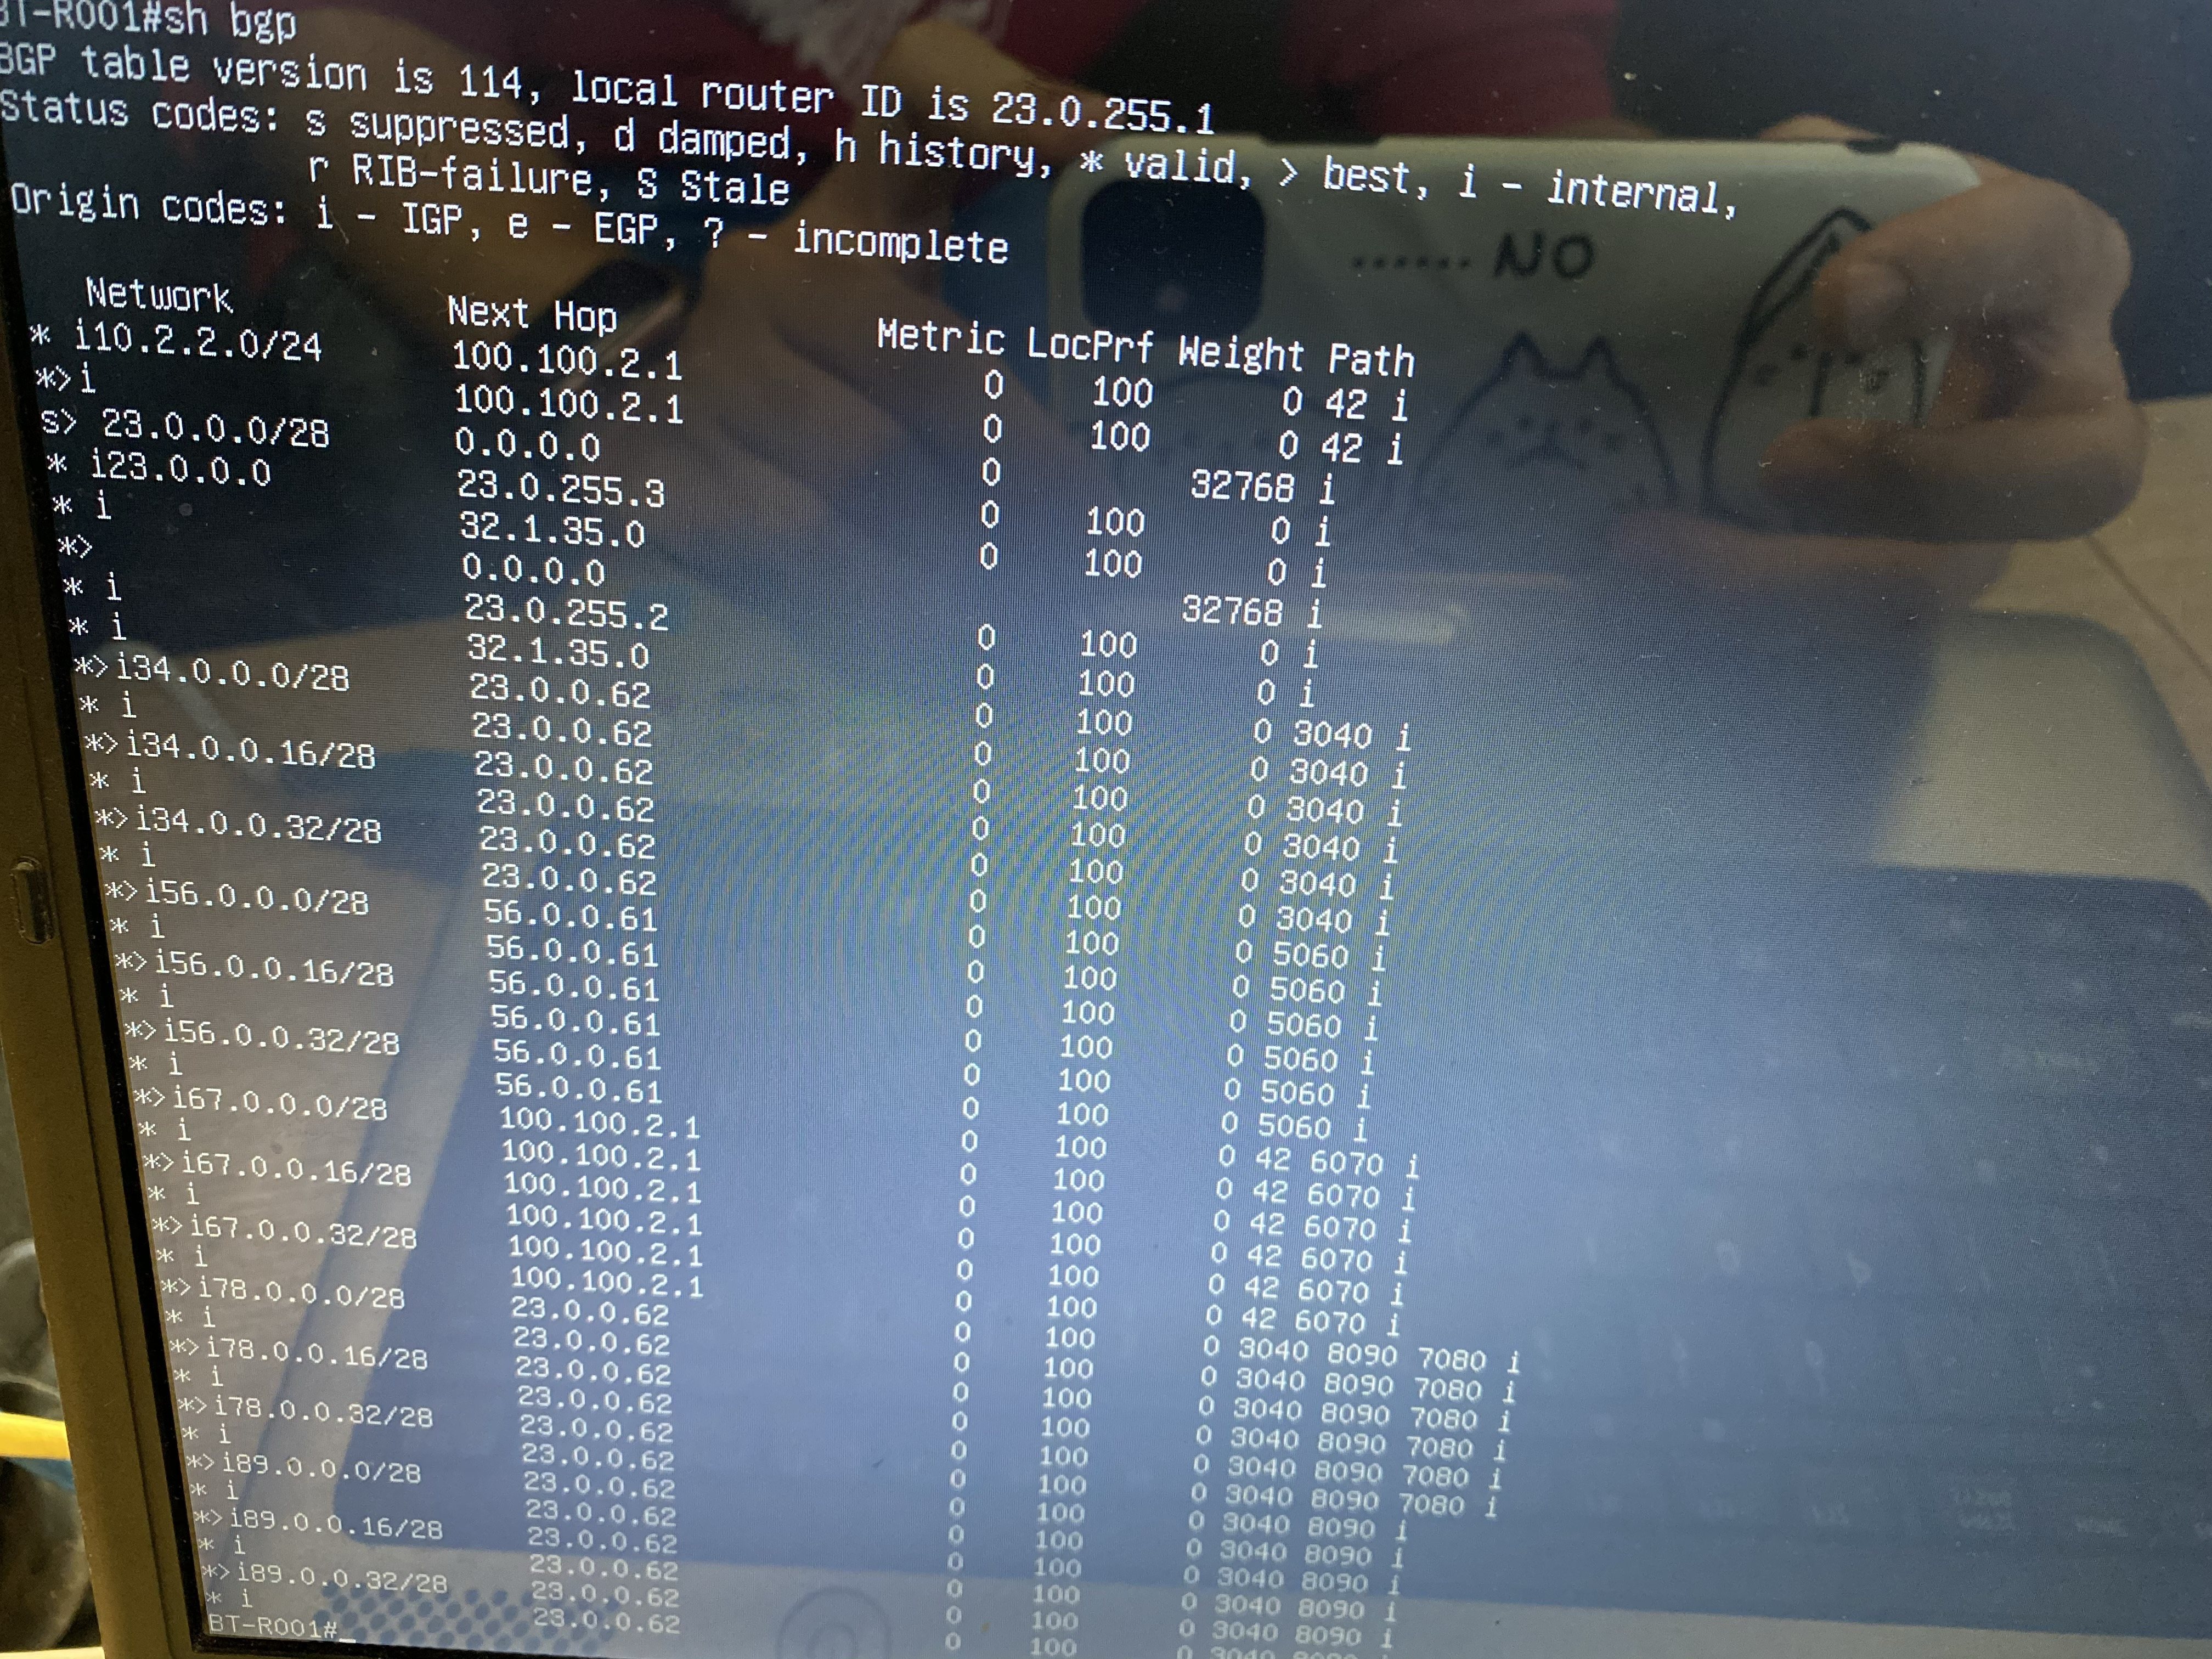
\includegraphics[width=\linewidth]{bgp-route-1}
        \caption{Router 1 (BT-R001)}
    \end{subfigure}
    \hfill
    \begin{minipage}[b]{0.3\textwidth}
	    \begin{subfigure}[b]{\linewidth}
	        \centering
	        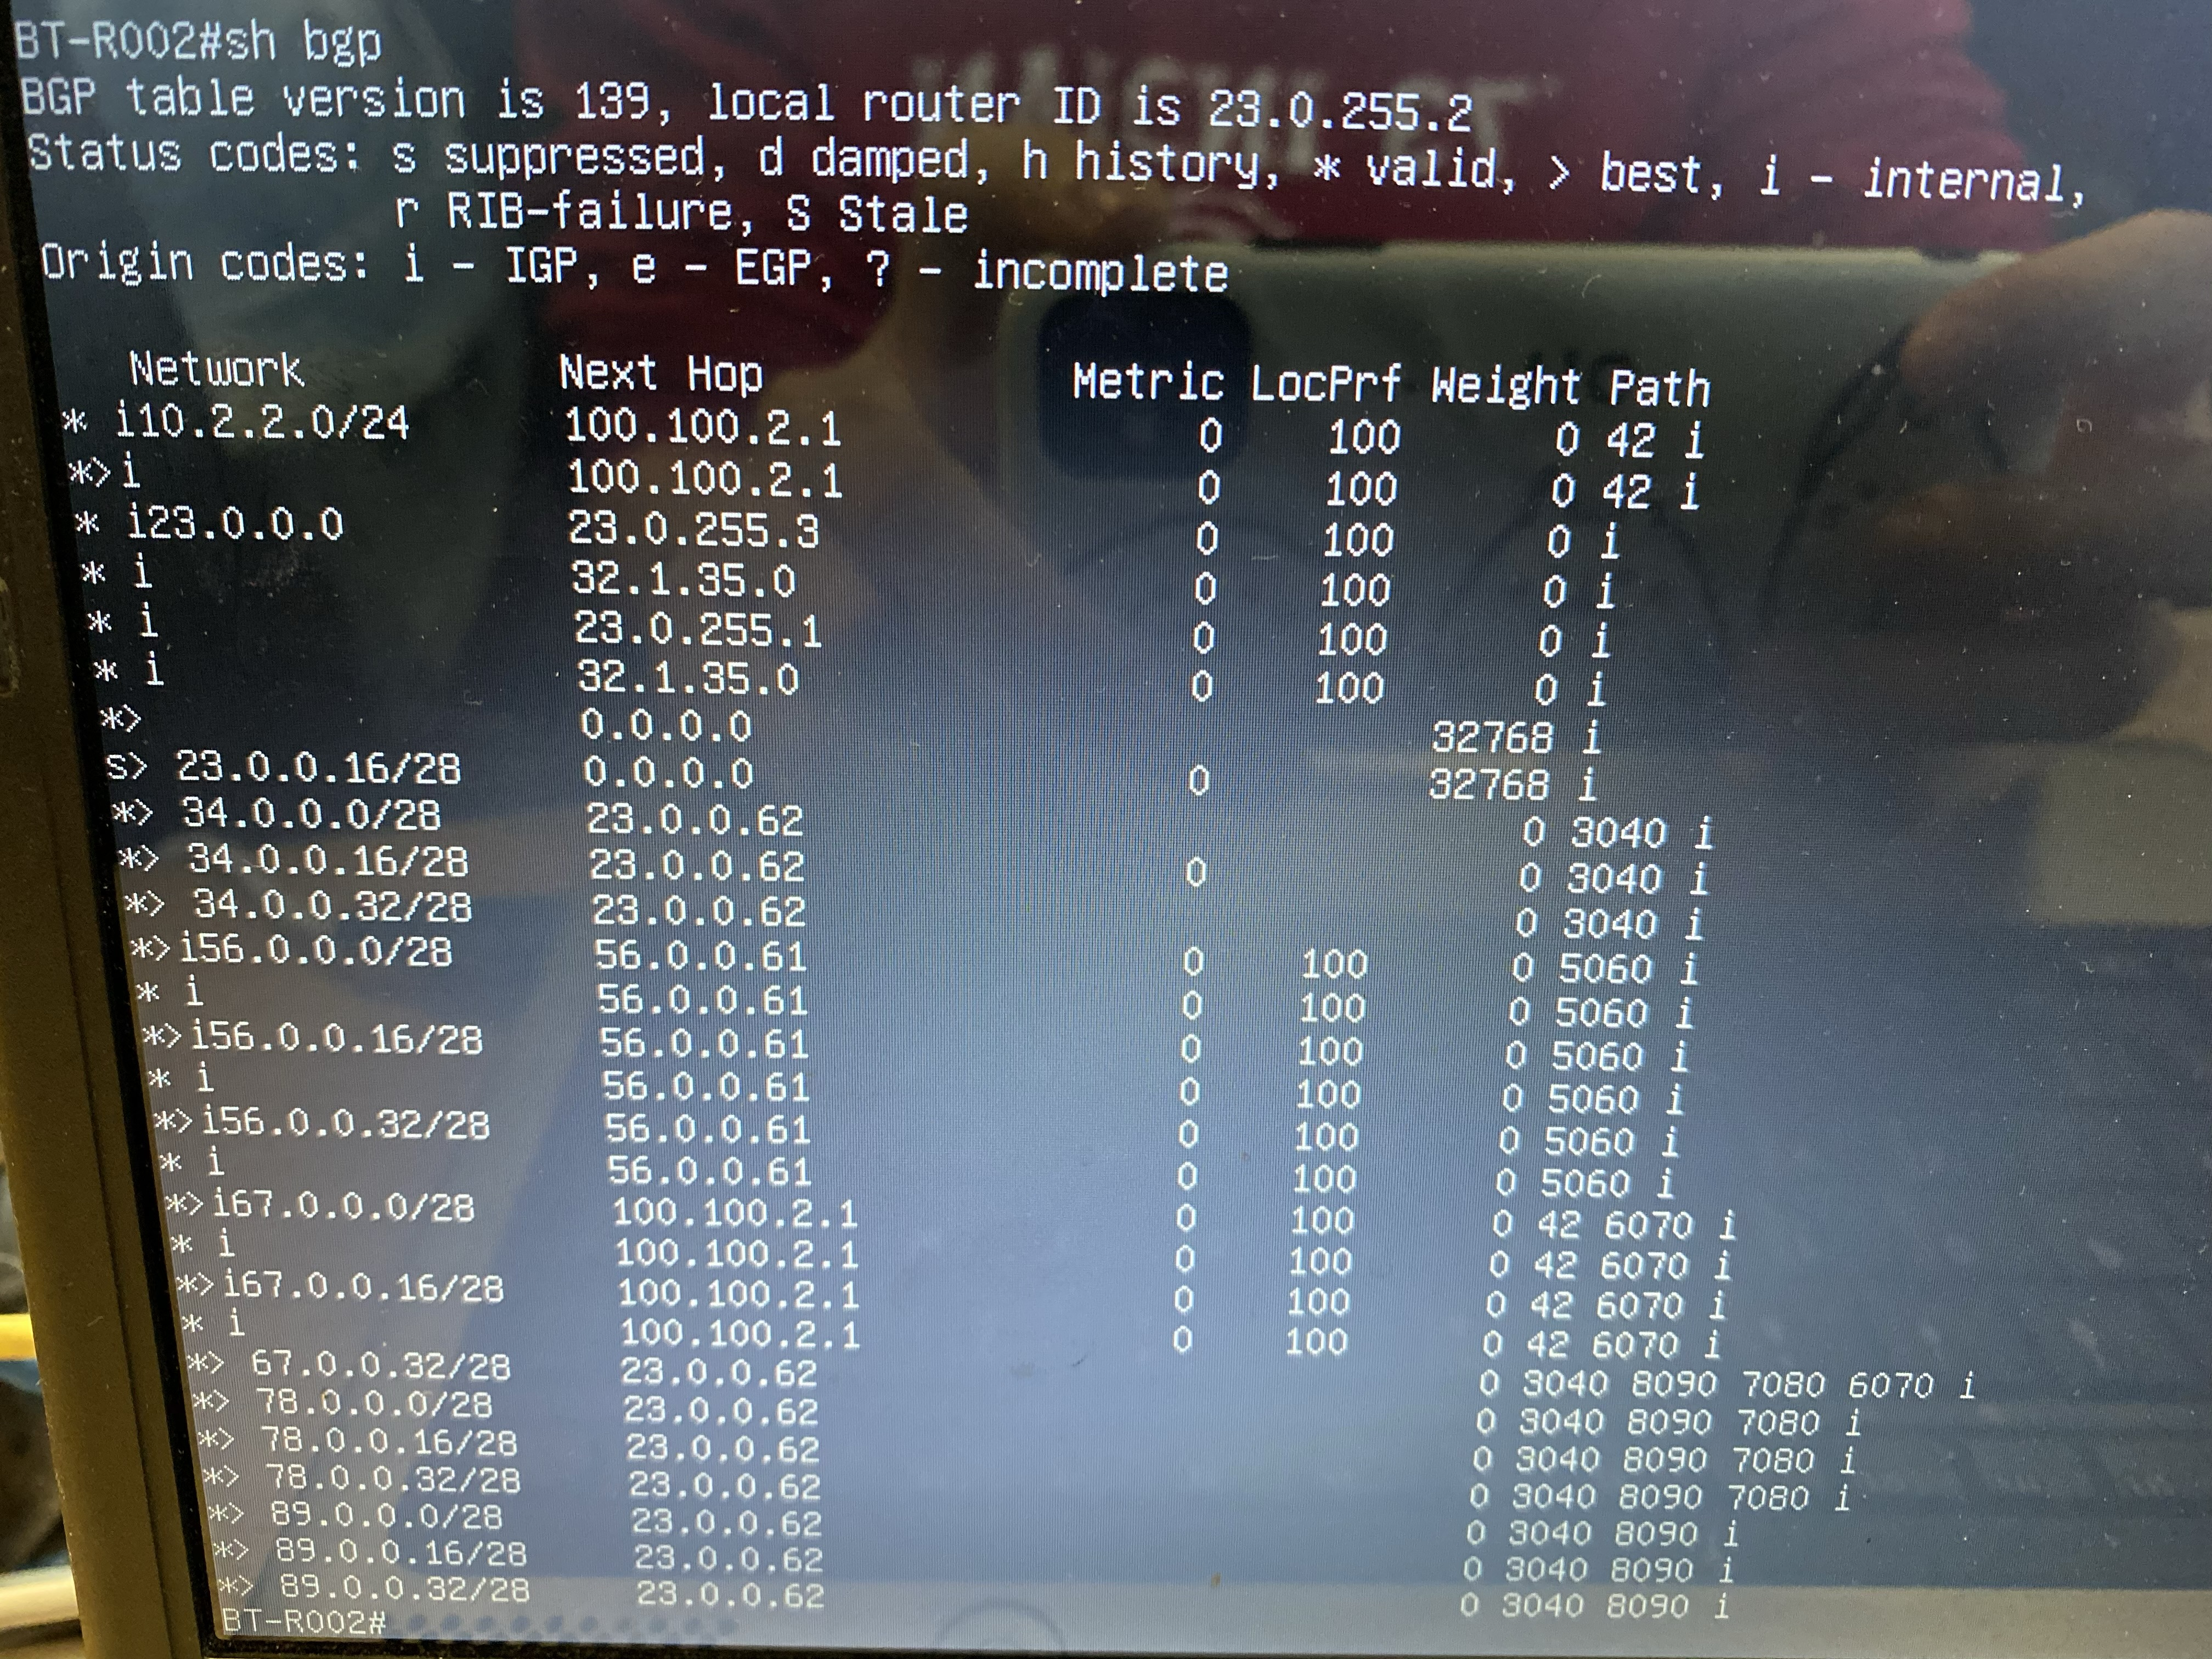
\includegraphics[width=\linewidth]{bgp-route-2}
	        \caption{Router 2 (BT-R002)}
	    \end{subfigure}
	    \\
	    \begin{subfigure}[b]{\linewidth}
	        \centering
	        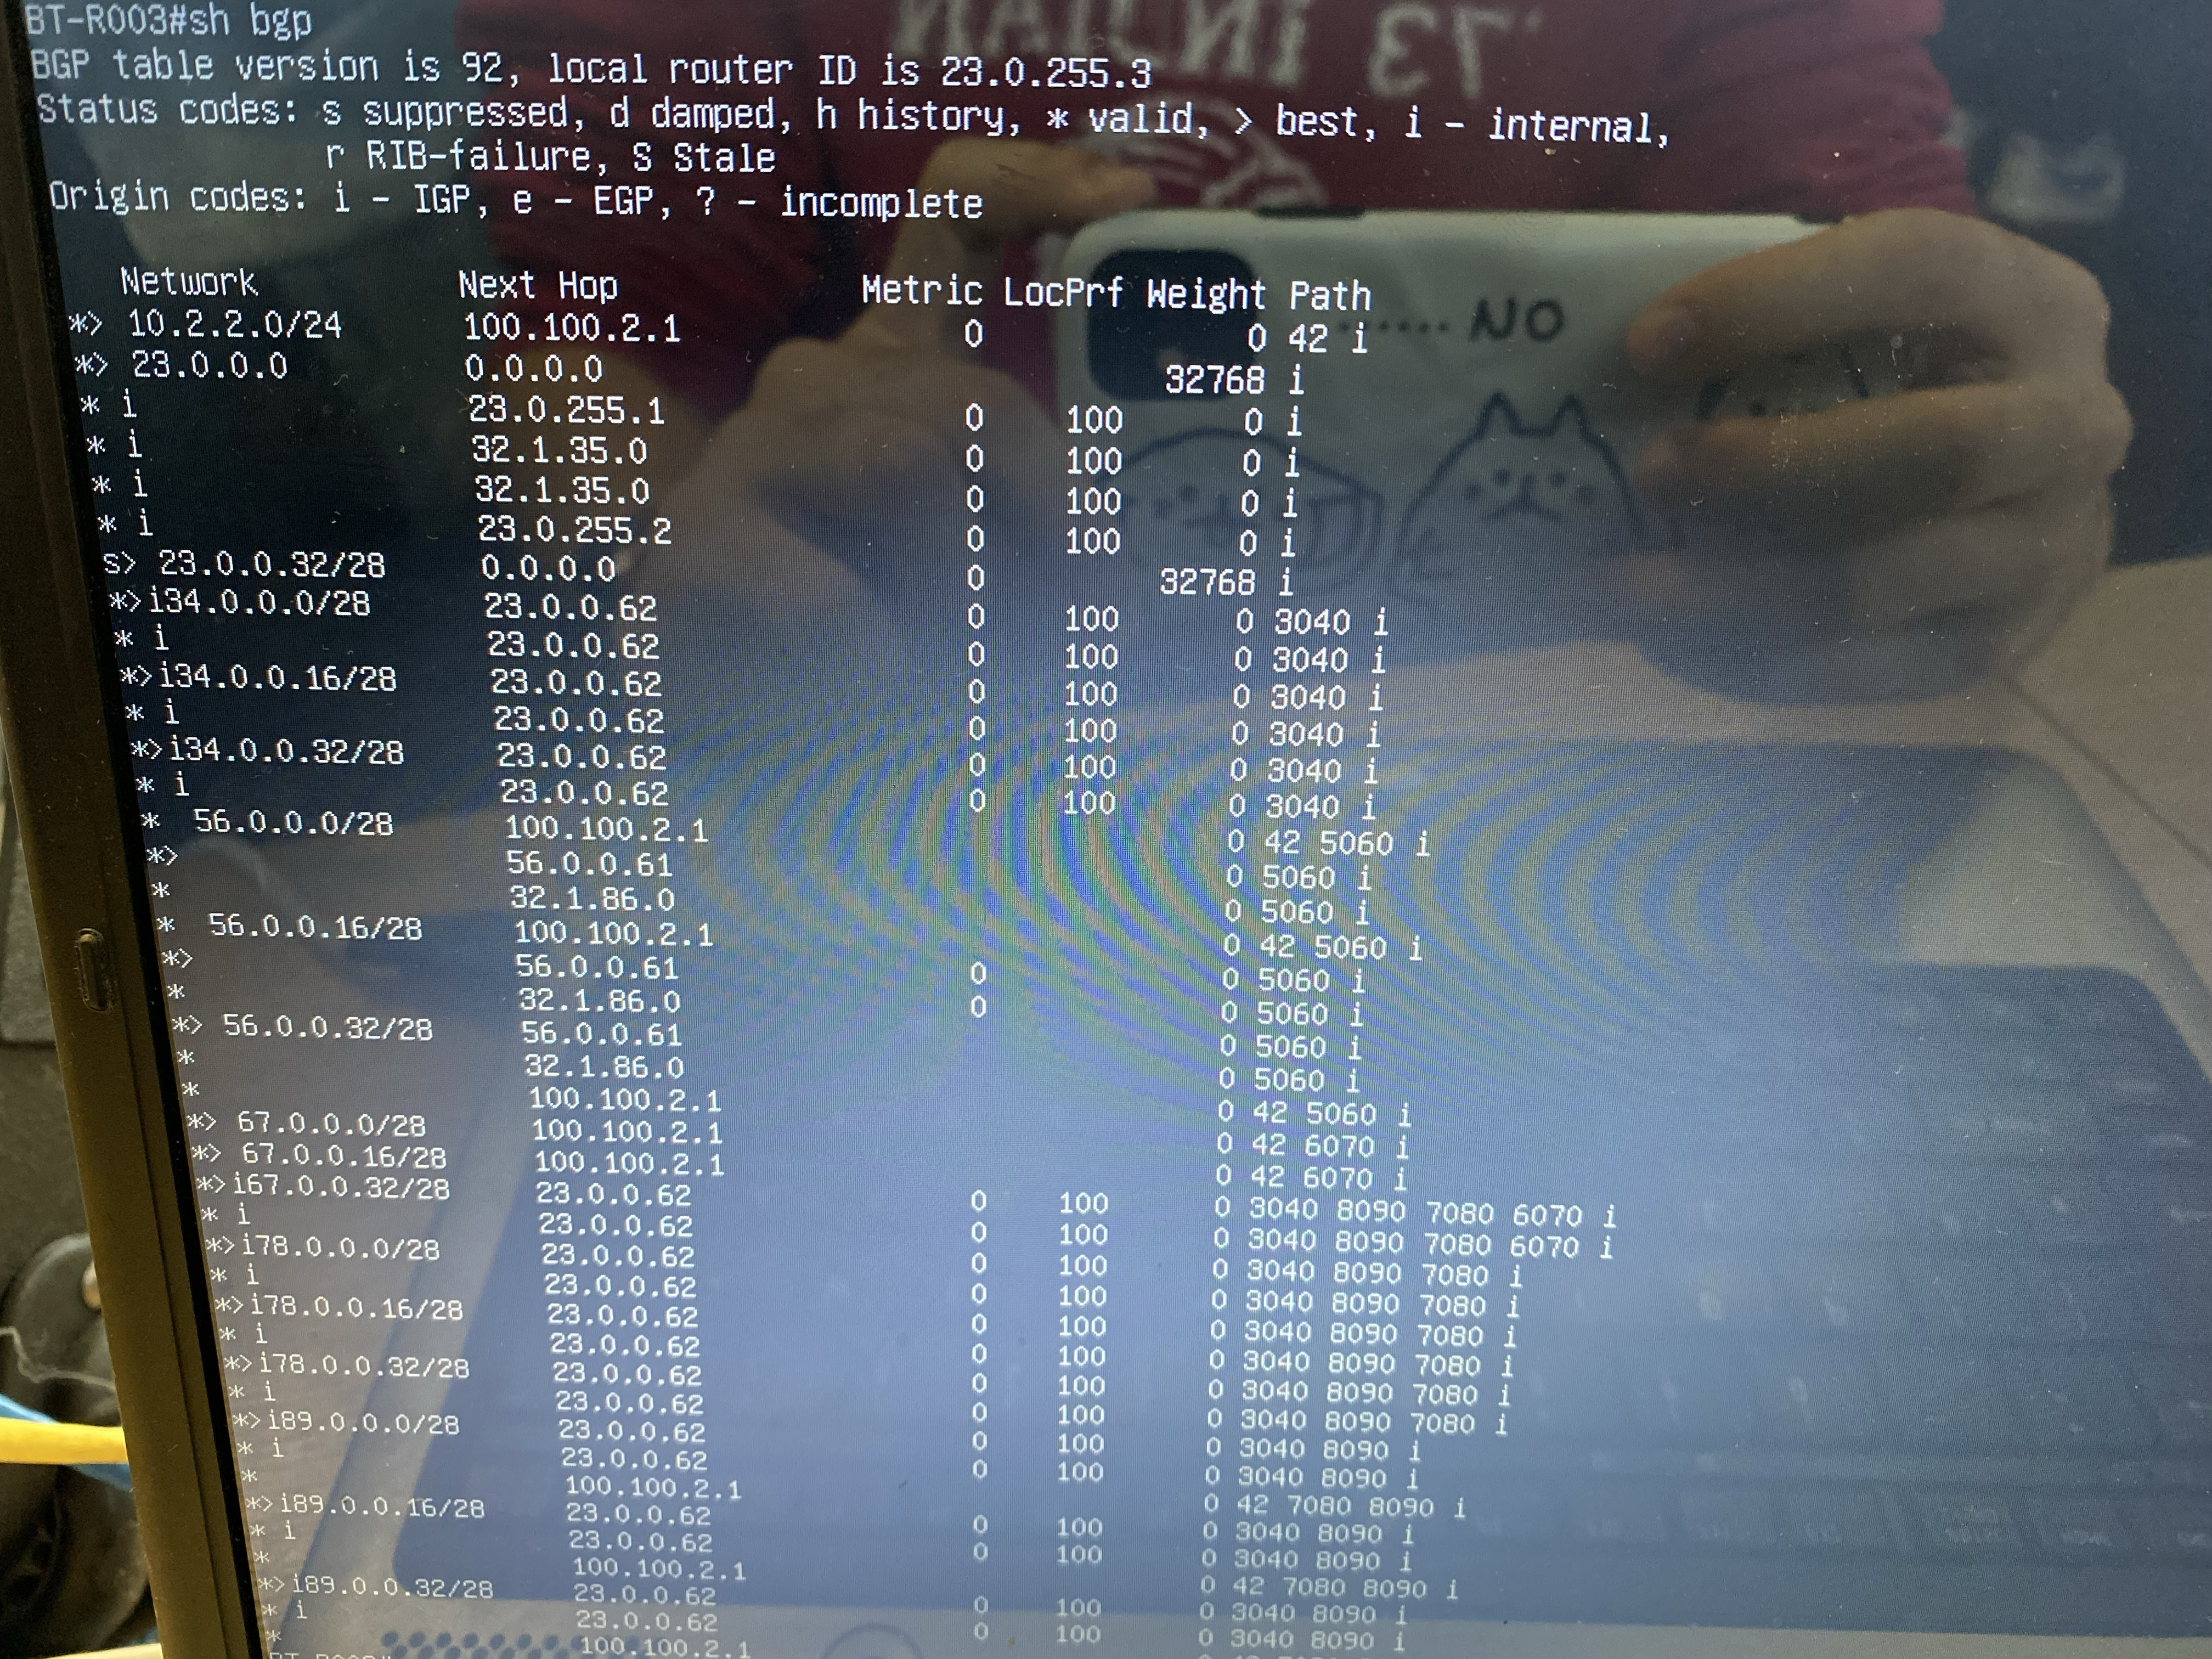
\includegraphics[width=\linewidth]{bgp-route-3}
	        \caption{Router 3 (BT-R003)}
	    \end{subfigure}
	\end{minipage}
    \caption{IPv4 Routes Collected through BGP Protocols on All $3$ Routers using \texttt{show bgp}.}
    \label{fig:bgp-route}
\end{figure*}



\clearpage


\subsubsection{Connectivity to Provider Central Network}

The connectivity to provider Central Network using BGP protocol is tested and evaluated by tracing routes to IP addresses \texttt{10.2.2.1} on Laptop 1 (BT001). As shown in Figure \ref{fig:bgp-central}, connection to Central Network is successfully established through BGP routes.

\begin{figure*}[ht!]
    \centering
    \begin{subfigure}[b]{\textwidth}
        \centering
        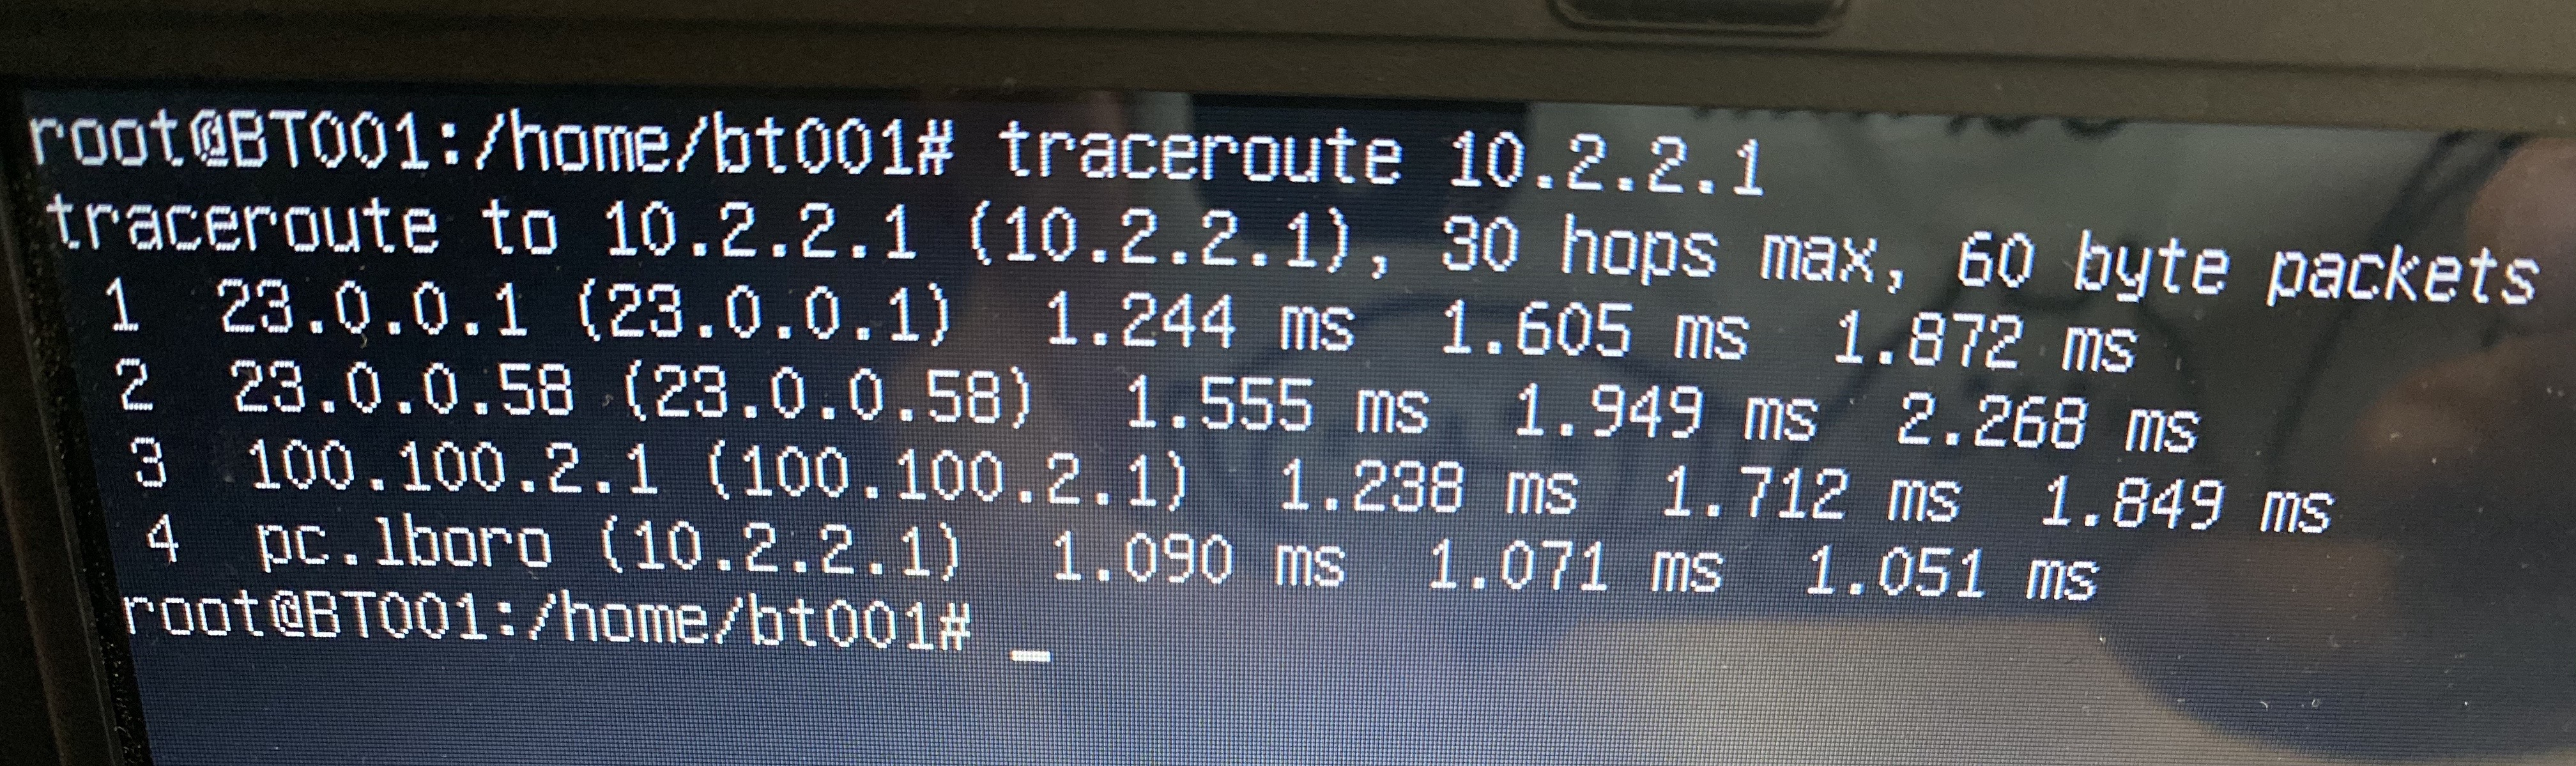
\includegraphics[width=\linewidth]{bgp-central-1}
        \caption{\texttt{10.2.2.1}}
    \end{subfigure}
    ~
    % \begin{subfigure}[b]{0.67\textwidth}
    %     \centering
    %     \includegraphics[width=\linewidth]{bgp-central-2}
    %     \caption{\texttt{10.2.2.253}}
    % \end{subfigure}
    \caption{Tracing IPv4 Routes to Central Network on Laptop 1 (BT001) using \texttt{traceroute}.}
    \label{fig:bgp-central}
\end{figure*}


\clearpage


\subsubsection{Connectivity to Customer DT Network}
The connectivity to customer DT Network using BGP protocol is tested and evaluated by tracing routes to IP addresses \texttt{34.0.0.2}, \texttt{34.0.0.18} and \texttt{34.0.0.34} on Laptop 1 (BT001). As shown in Figure \ref{fig:bgp-dt}, connection to DT Network is successfully established through BGP routes.

\begin{figure*}[ht!]
    \centering
    \begin{subfigure}[b]{\textwidth}
        \centering
        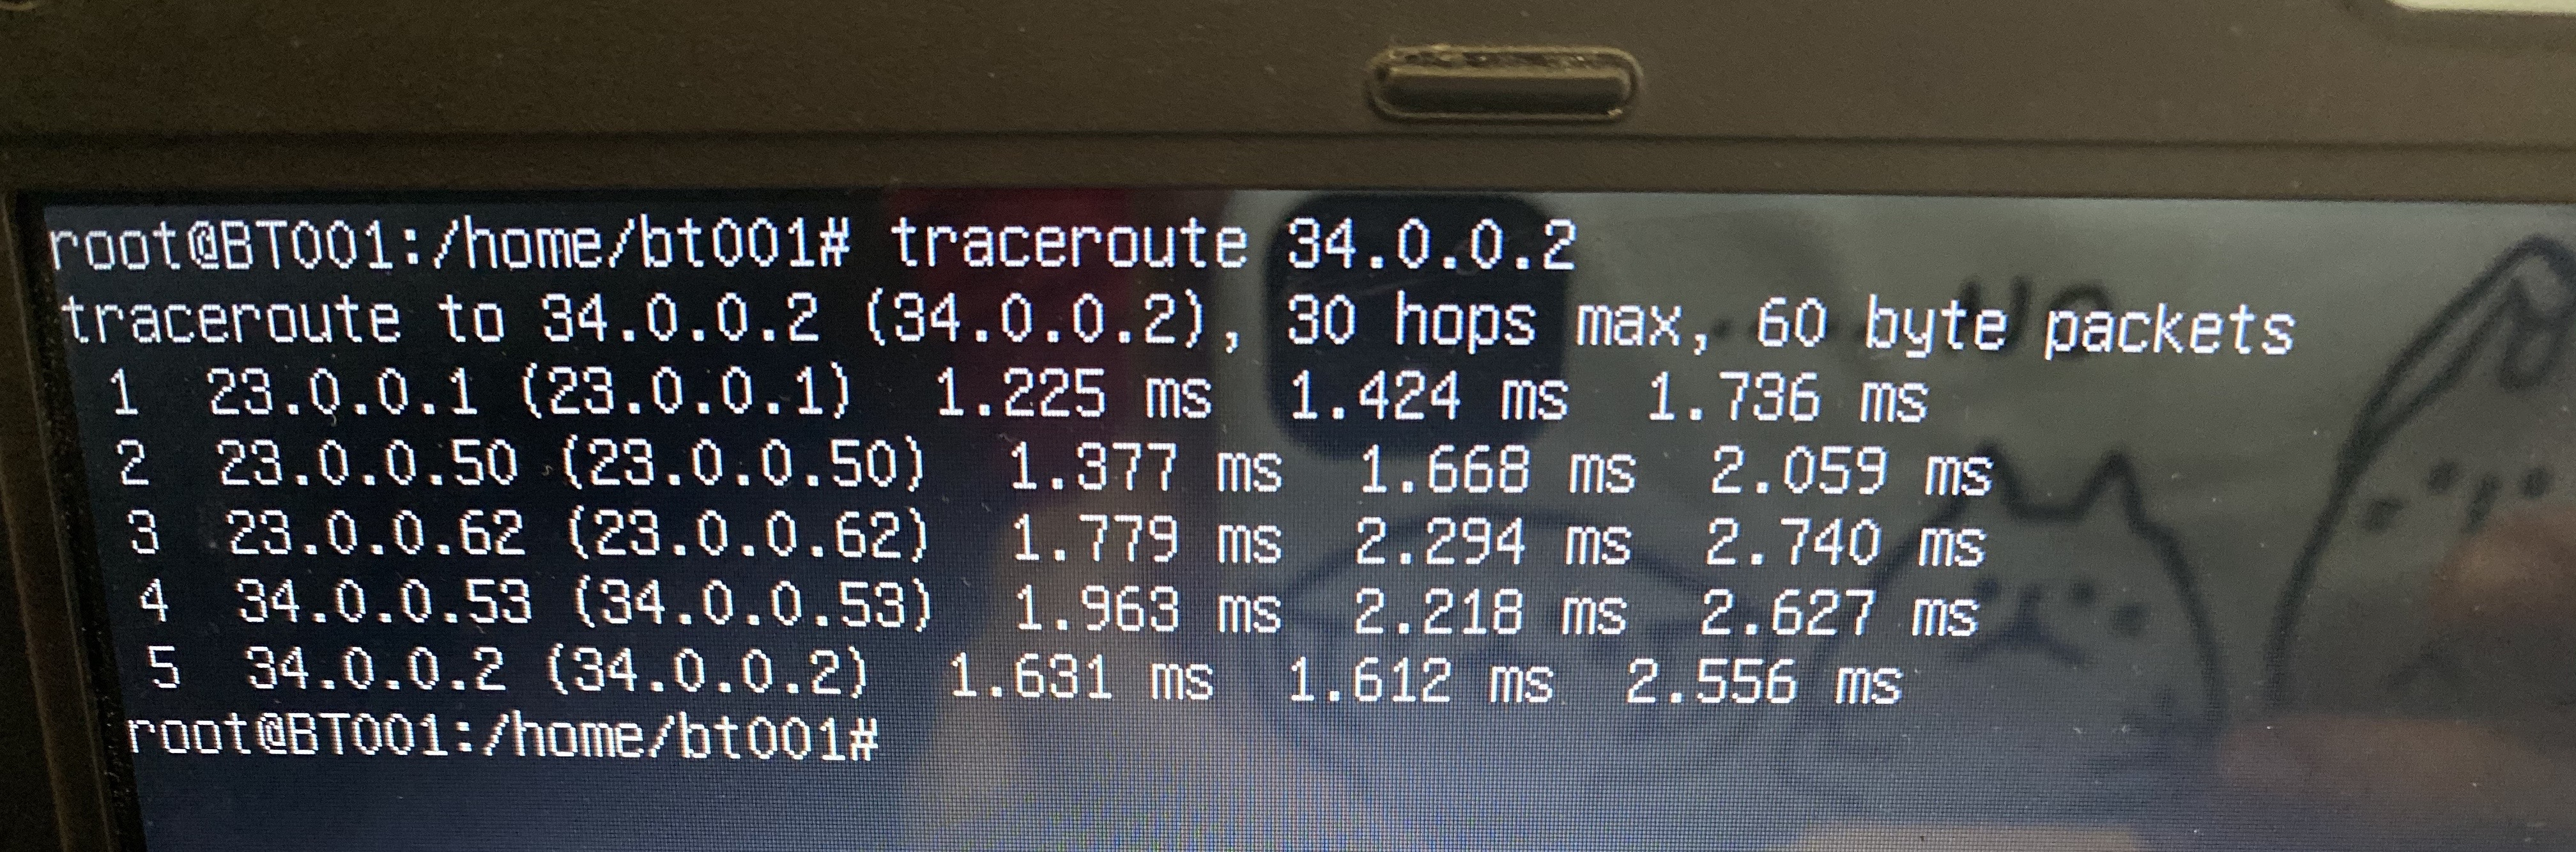
\includegraphics[width=\linewidth]{bgp-dt-1}
        \caption{\texttt{34.0.0.2}}
    \end{subfigure}
    ~
    \begin{subfigure}[b]{\textwidth}
        \centering
        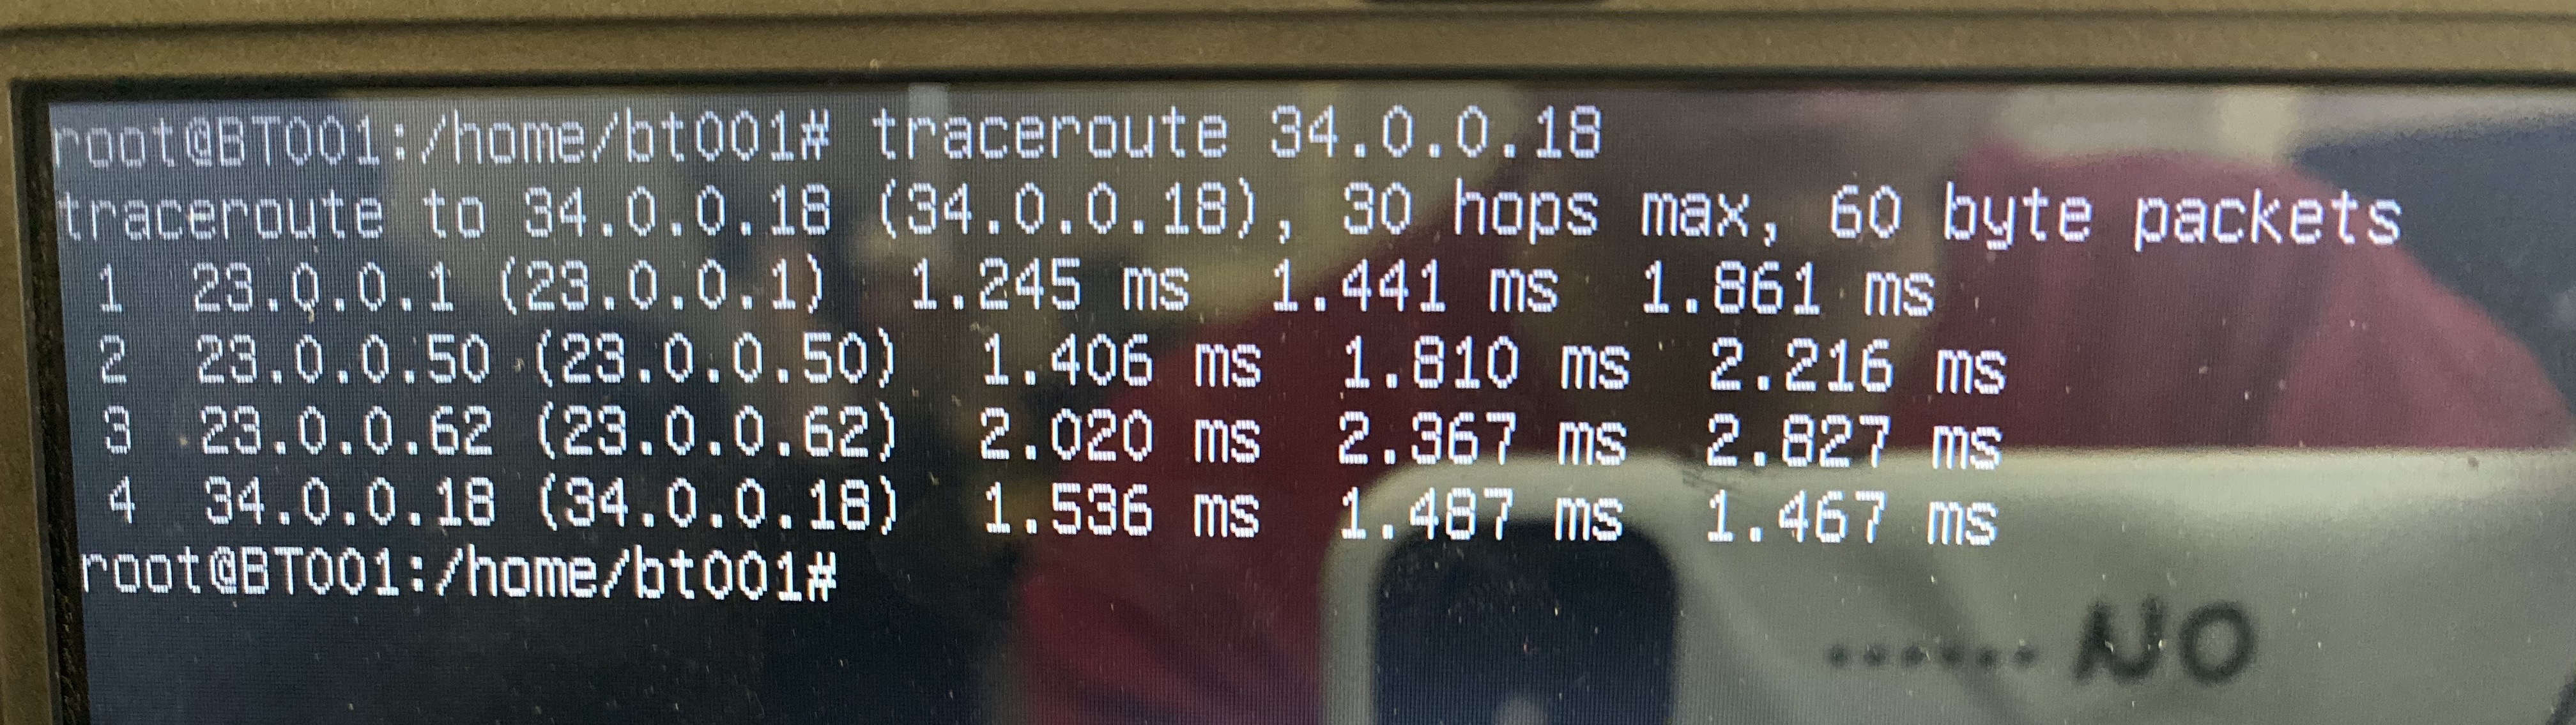
\includegraphics[width=\linewidth]{bgp-dt-2}
        \caption{\texttt{34.0.0.18}}
    \end{subfigure}
    ~
    \begin{subfigure}[b]{\textwidth}
        \centering
        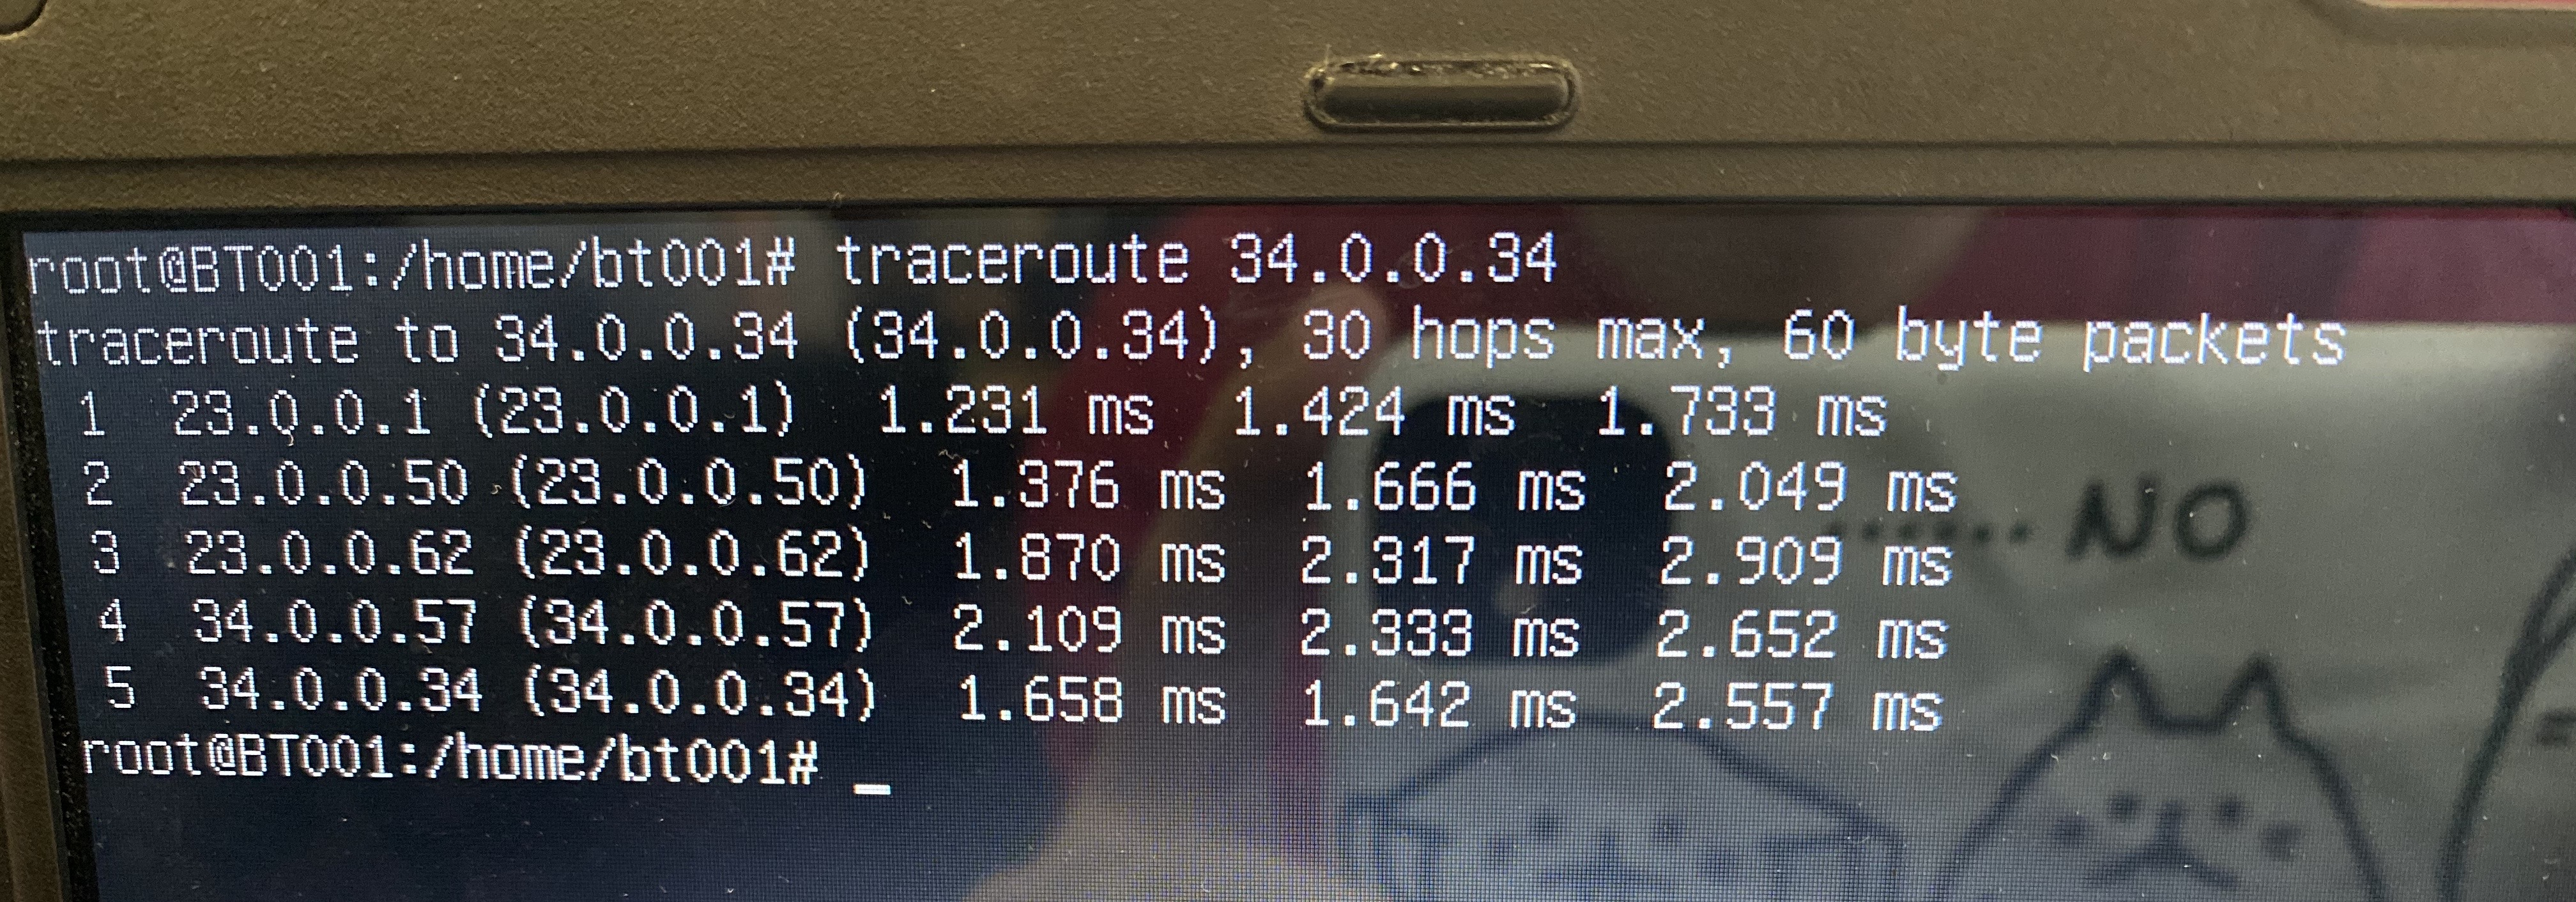
\includegraphics[width=\linewidth]{bgp-dt-3}
        \caption{\texttt{34.0.0.34}}
    \end{subfigure}
    ~
    \caption{Tracing IPv4 Routes to DT Network on Laptop 1 (BT001) using \texttt{traceroute}.}
    \label{fig:bgp-dt}
\end{figure*}



\clearpage

\subsubsection{Connectivity to Peer Virgin Network}
The connectivity to peer Virgin Network using BGP protocol is tested and evaluated by tracing routes to IP addresses \texttt{56.0.0.2}, \texttt{56.0.0.18} and \texttt{56.0.0.34} on Laptop 1 (BT001). As shown in Figure \ref{fig:bgp-virgin}, connection to Virgin Network is successfully established through BGP routes.

\begin{figure*}[ht!]
    \centering
    \begin{subfigure}[b]{\textwidth}
        \centering
        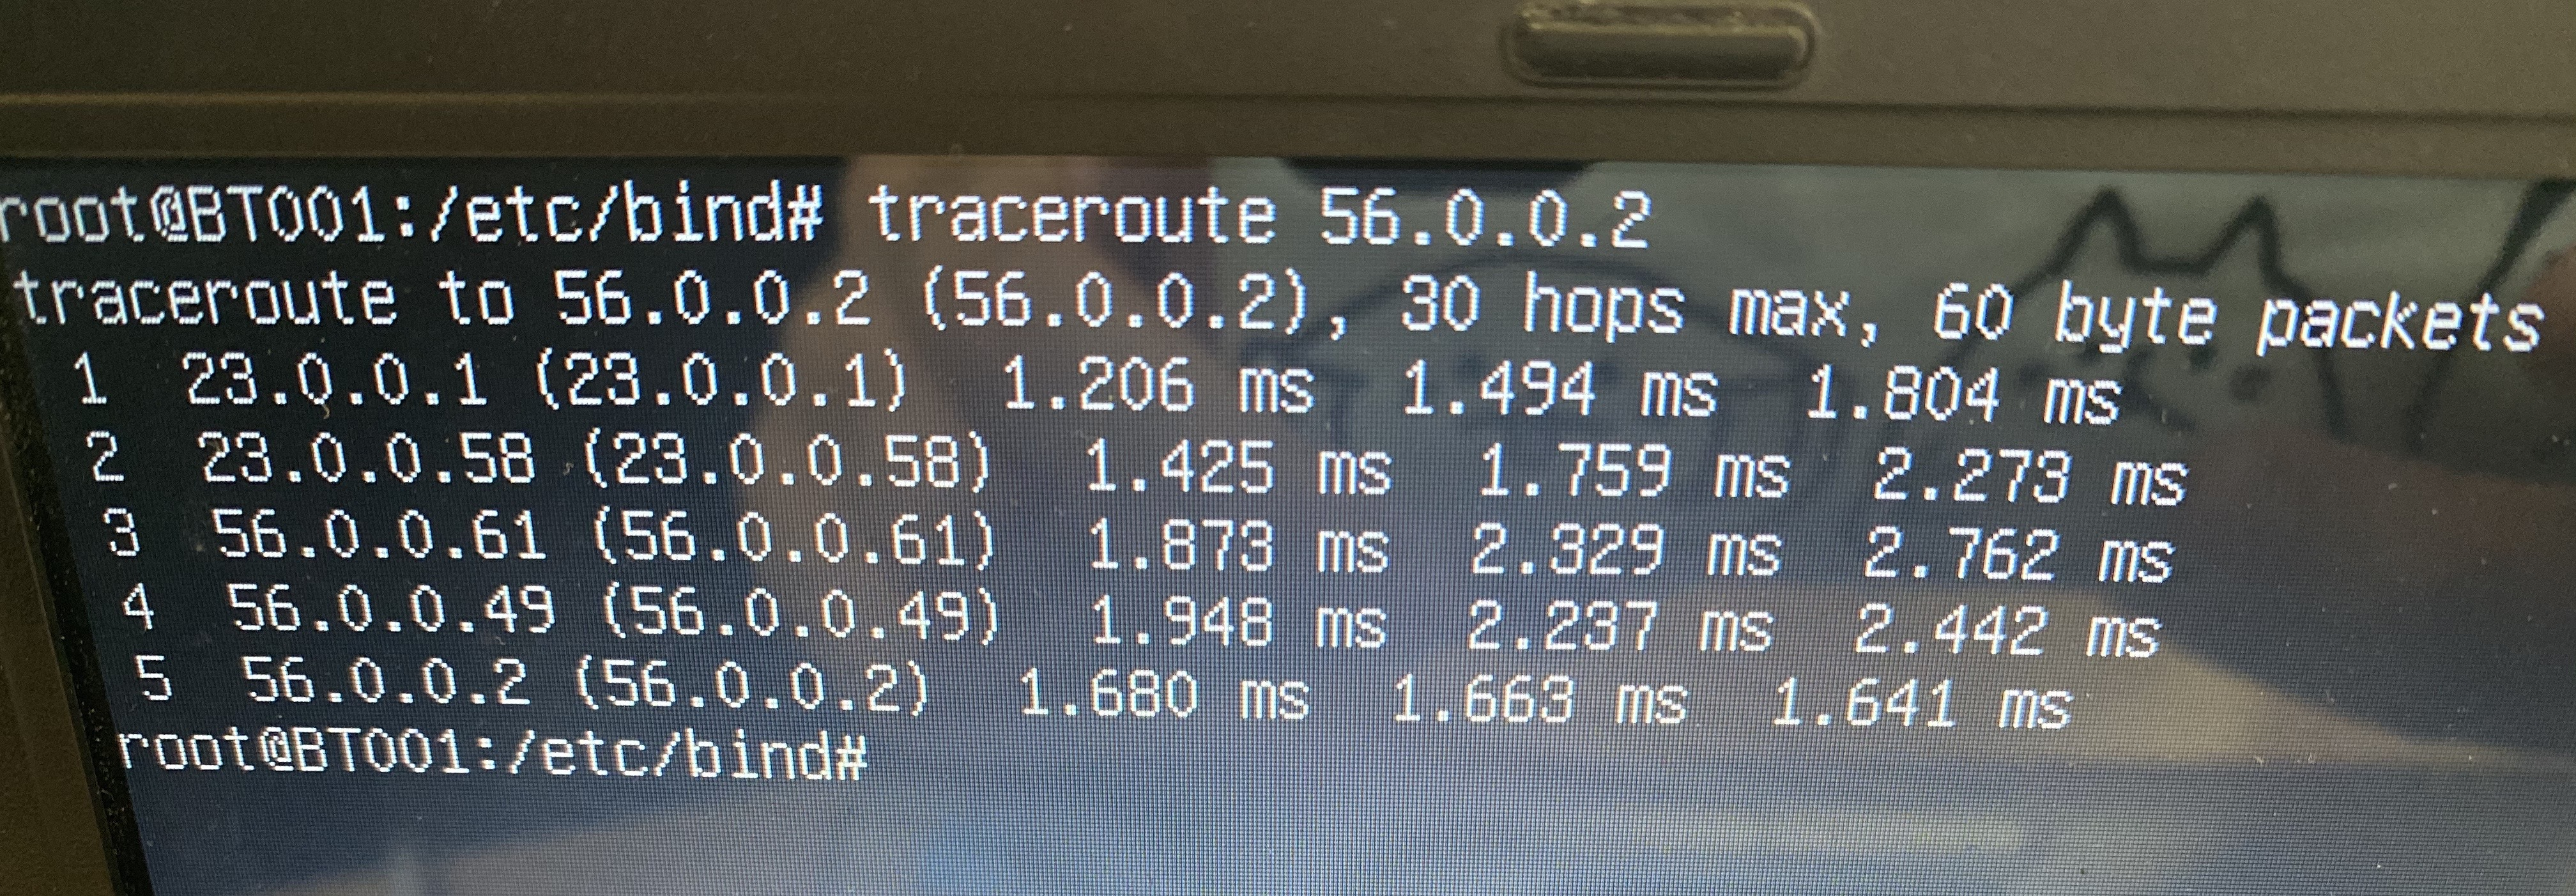
\includegraphics[width=\linewidth]{bgp-virgin-1}
        \caption{\texttt{56.0.0.2}}
    \end{subfigure}
    ~
    \begin{subfigure}[b]{\textwidth}
        \centering
        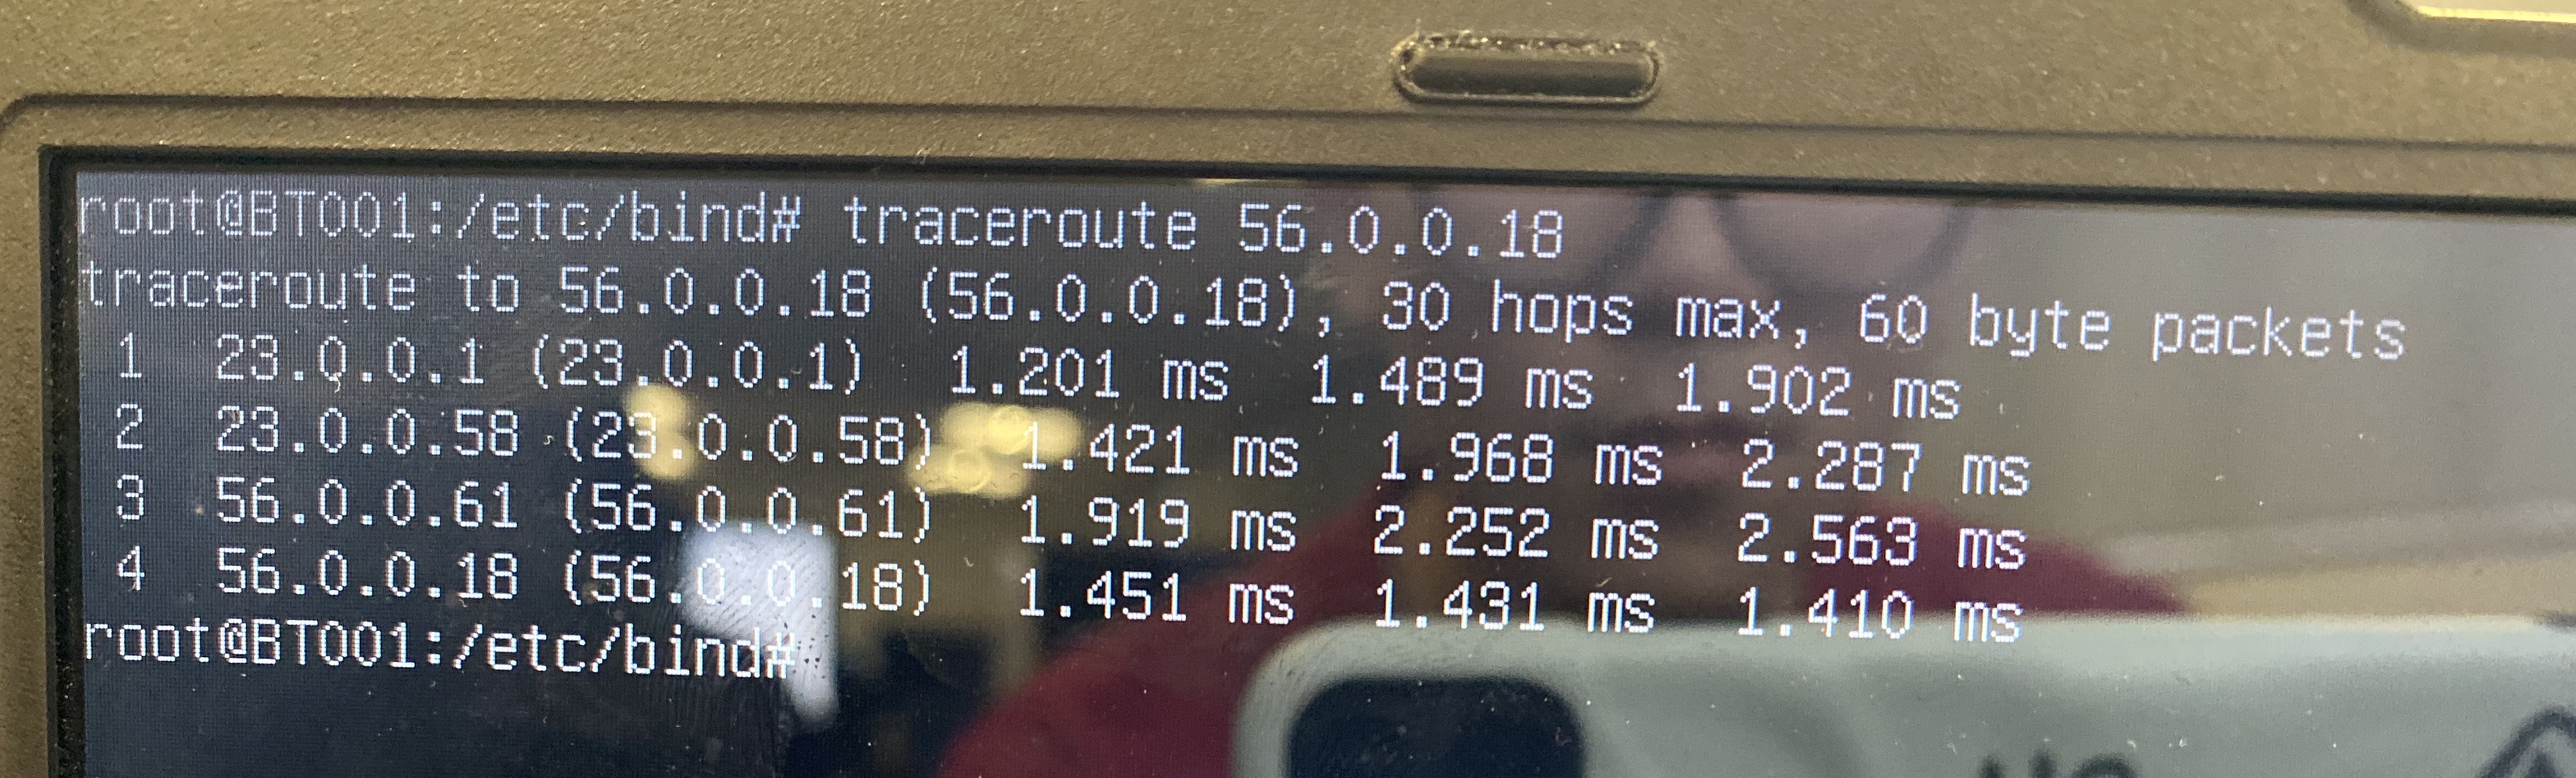
\includegraphics[width=\linewidth]{bgp-virgin-2}
        \caption{\texttt{56.0.0.18}}
    \end{subfigure}
    ~
    \begin{subfigure}[b]{\textwidth}
        \centering
        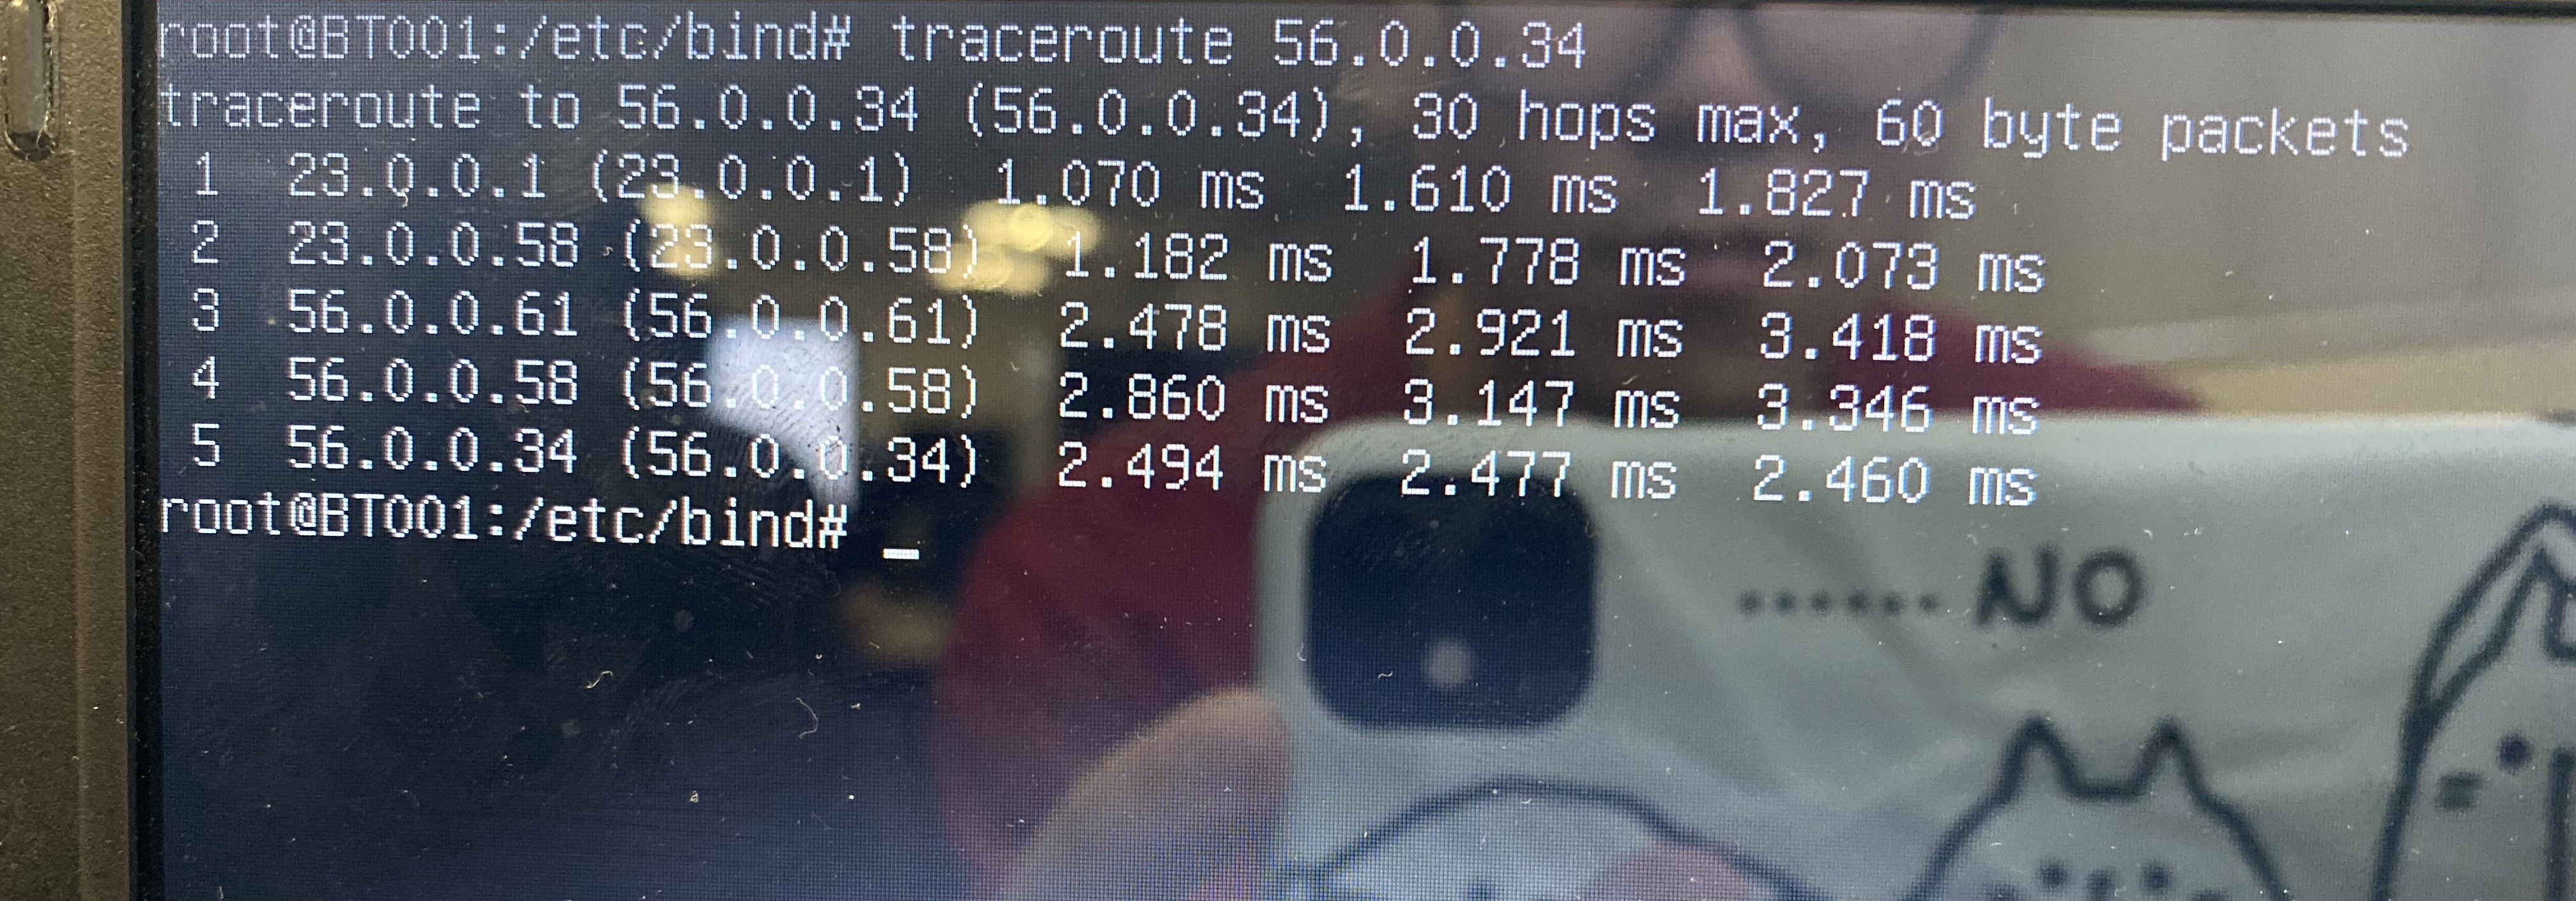
\includegraphics[width=\linewidth]{bgp-virgin-3}
        \caption{\texttt{56.0.0.34}}
    \end{subfigure}
    ~
    \caption{Tracing IPv4 Routes to Virgin Network on Laptop 1 (BT001) using \texttt{traceroute}.}
    \label{fig:bgp-virgin}
\end{figure*}



\clearpage


\subsubsection{Connectivity to Other Networks}
The connectivity to other networks using BGP protocol is tested and evaluated by tracing routes to IP addresses \texttt{78.0.0.2} (Sonara Network) and \texttt{89.0.0.18} (NTT Network) on Laptop 1 (BT001). As shown in Figure \ref{fig:bgp-virgin}, connection to Virgin Network is successfully established through BGP routes.

\begin{figure*}[ht!]
    \centering
    \begin{subfigure}[b]{\textwidth}
        \centering
        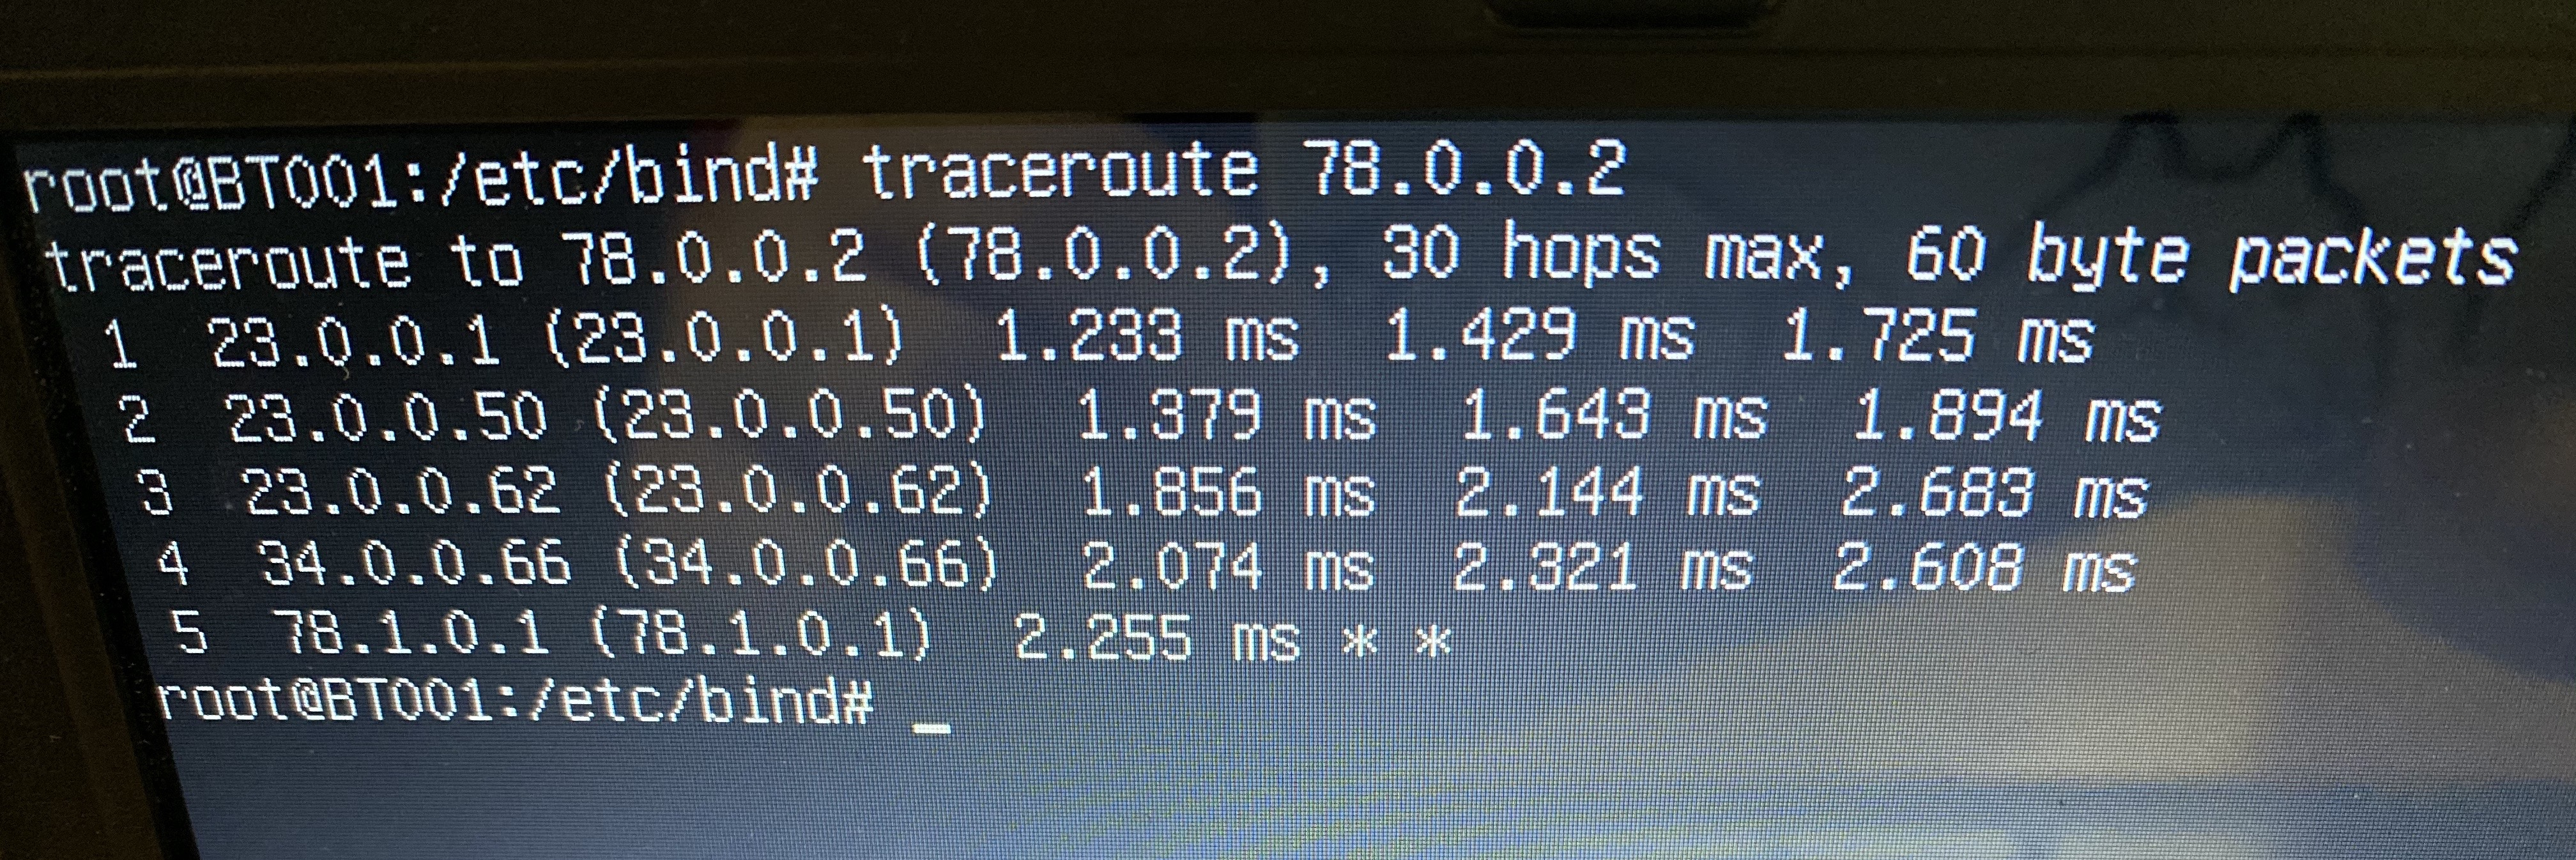
\includegraphics[width=\linewidth]{bgp-other-1}
        \caption{\texttt{78.0.0.2}}
    \end{subfigure}
    ~
    \begin{subfigure}[b]{\textwidth}
        \centering
        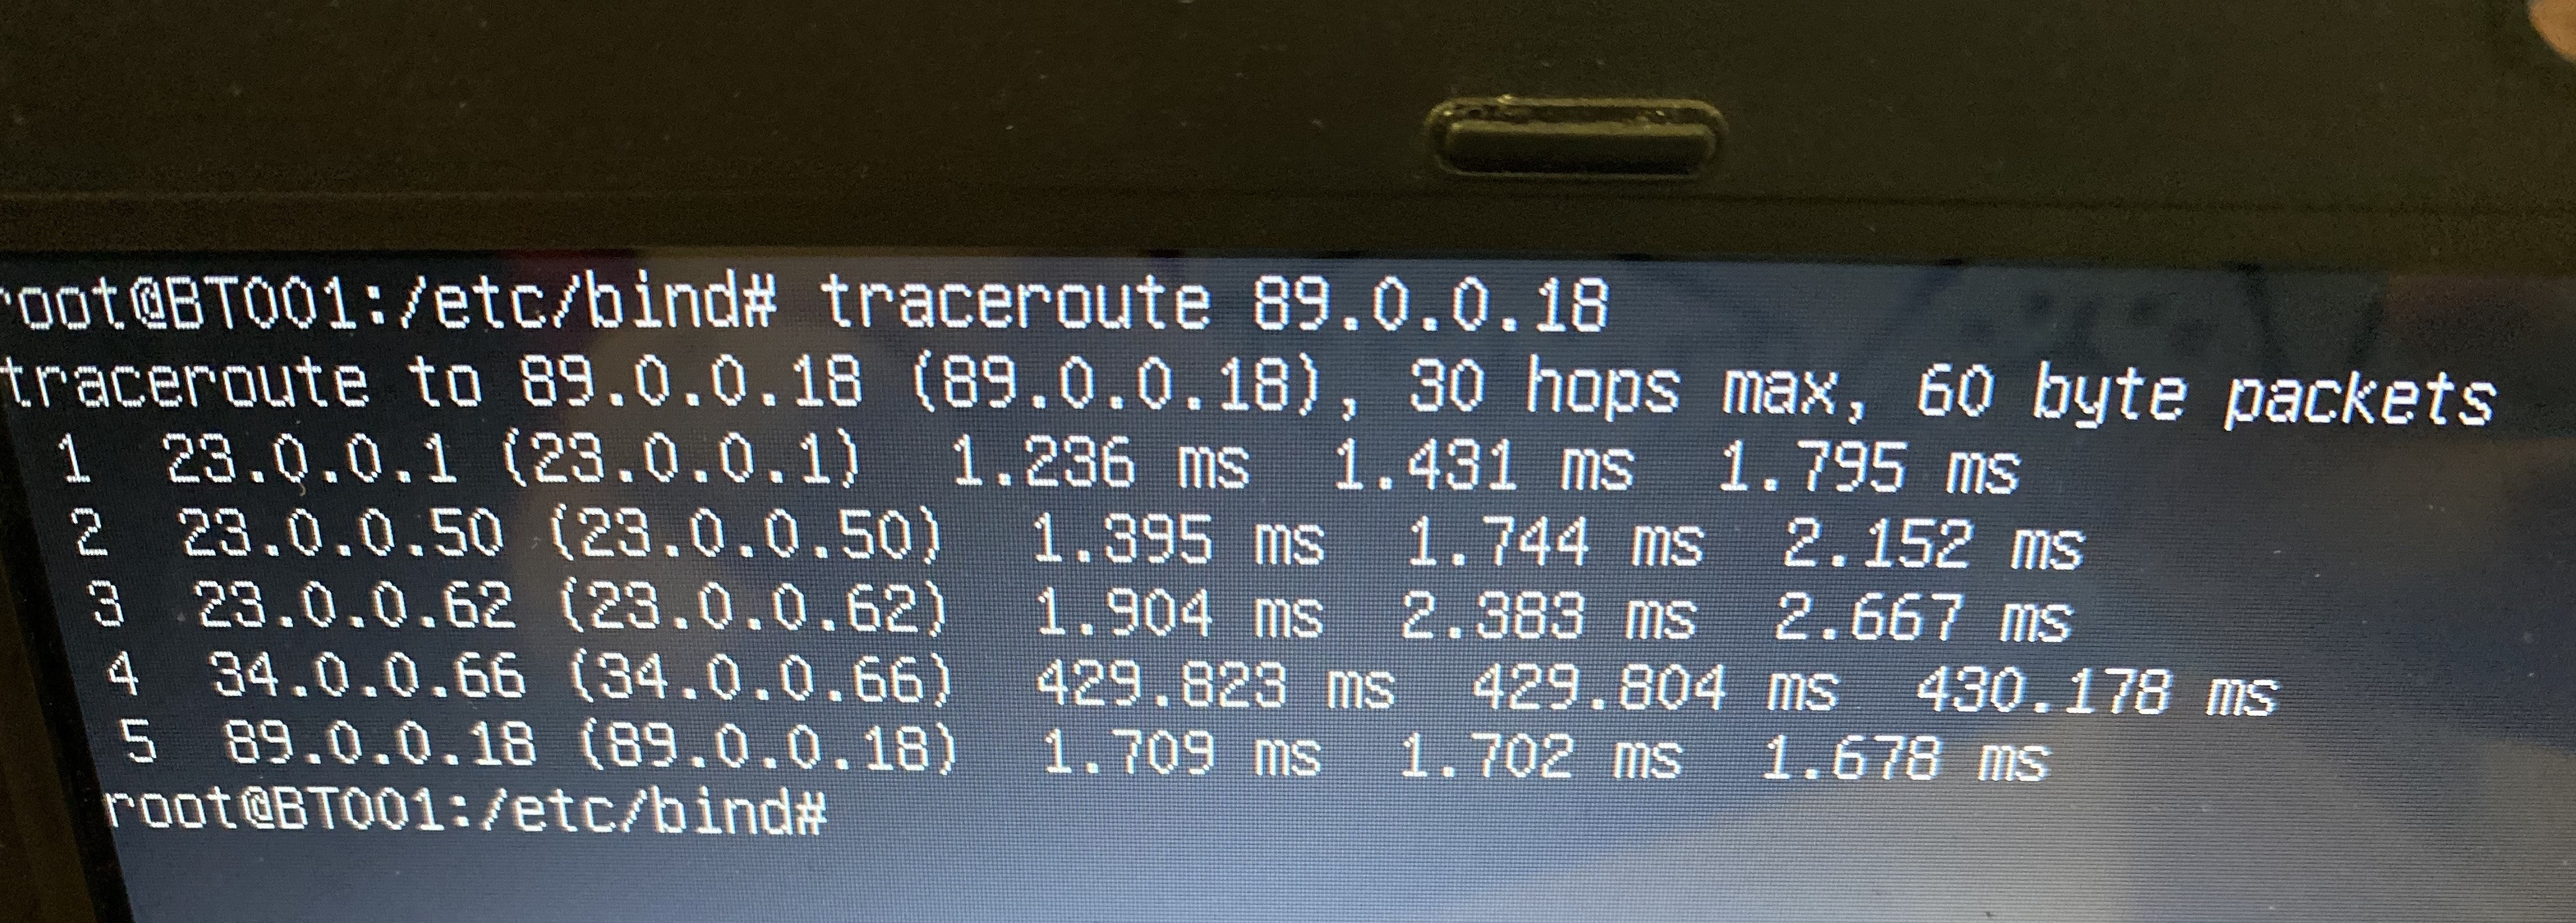
\includegraphics[width=\linewidth]{bgp-other-2}
        \caption{\texttt{89.0.0.18}}
    \end{subfigure}
    \caption{Tracing IPv4 Routes to Other Networks on Laptop 1 (BT001) using \texttt{traceroute}.}
    \label{fig:bgp-virgin}
\end{figure*}



\clearpage


\subsection{Commentary}

\subsubsection{Problem: Filter List Not Working for Self-Originated Routes}

The initial filter list for outbound routes on Router 3 only permits routes originated from BT Network (ASN 2030) and customer DT Network (ASN 3040).

\begin{lstlisting}
ip as-path access-list 1 permit _2030$
ip as-path access-list 1 permit _3040$
\end{lstlisting}

However, the filter list blocks all routes except those originated from customer DT Network to be announced. To solve this problem, a filter list where all routes except those go through provider Central Network (ASN 42) and peer Virgin Network (ASN 5060) are allowed. The new list should have the same effects as the previous list and indeed works as intended.

\begin{lstlisting}
ip as-path access-list 1 deny _42_
ip as-path access-list 1 deny _5060_
ip as-path access-list 1 permit .*
\end{lstlisting}

% \subsubsection{Problem: Loopback Addresses}



